% !TeX spellcheck = sv_SE
%http://www.cs.put.poznan.pl/ksiek/latexmath.html
%https://en.wikibooks.org/wiki/LaTeX/Advanced_Mathematics
%http://www.maths.lth.se/matematiklth/personal/magnusa/kurser/endim-ht2015/B1/kurspmB1ht15.pdf

\documentclass[a4paper]{article} 
\usepackage[T1]{fontenc} 
\usepackage[utf8]{inputenc} 
\usepackage[swedish]{babel} 
\usepackage{amsmath}
\usepackage{amssymb}
\usepackage{cancel}
\usepackage{graphicx}

\usepackage{color}
\definecolor{tskcol}{RGB}{193,70,70}
\newcommand{\tskcol}[1]{\textcolor{tskcol}{#1}}

\setlength{\parindent}{0in}

\title{Endimensionell analys\\ HT-2015} 
\author{Emil Wihlander\\ dat15ewi@student.lu.se} 
\date{2015--09--23}

\begin{document}
	\maketitle
	\pagebreak
	
	\section*{Kapitel 1: Grundläggande begrepp och terminologi}
	Om jag skriver ''alla tal'' syftar jag på alla reella tal.
	\subsection*{Talsystem}
	\texttt{\tskcol{1.1~~~a) (s. 1)}}
	\begin{quotation}
		\noindent
		De naturliga talen ($\mathbb{N}$) innefattar alla heltal som är noll eller större. $\tfrac{6}{2}=3,~\tfrac{3}{0.1}=30,~\tfrac{0}{5}=0$.
		\\ \\
		\textbf{Svar}: 
		\[\frac{6}{2},~0,~3,~\frac{3}{0.1},~\frac{0}{5}\]
	\end{quotation}
	
	\texttt{\tskcol{~~~~~~b) (s. 1)}}
	\begin{quotation}
		\noindent
		De hela talen ($\mathbb{Z}$) inkluderar de naturliga talen ($\mathbb{N}$) samt alla negativa heltal. $-\frac{0.3}{0.02}=-15$.
		\\ \\
		\textbf{Svar}: 
		\[\frac{6}{2},~0,~3,~-3,~\frac{3}{0.1},~-\frac{0.3}{0.02},~\frac{0}{5}\]
	\end{quotation}
	
	\texttt{\tskcol{~~~~~~c) (s. 2)}}
	\begin{quotation}
		\noindent
		Rationella tal ($\mathbb{Q}$) är tal som kan skrivas som bråk (inkluderar de hela talen ($\mathbb{Z}$)). $3=\frac{3}{1}$ osv...
		\\ \\
		\textbf{Svar}: 
		\[\frac{6}{2},~0,~3,~-3,~\frac{3}{0.1},~\frac{3}{5},~\frac{5}{3}~-\frac{0.3}{0.02},~\frac{0}{5}\]
	\end{quotation}

	\texttt{\tskcol{~~~~~~d) (s. 2)}}
	\begin{quotation}
		\noindent
		Reella tal ($\mathbb{R}$) är alla ''vanliga'' tal (inte de komplexa talen ($\mathbb{C}$)).
		\\ \\
		\textbf{Svar}: 
		\[\frac{6}{2},~0,~3,~-3,~\frac{3}{0.1},~\frac{3}{5},~\frac{5}{3},~\sqrt{2},~-\frac{0.3}{0.02},~\frac{0}{5},~\pi\]
	\end{quotation}
	
	\texttt{\tskcol{1.2 (saknar sida)}}
	\begin{quotation}
		\noindent
		Alla tal med ändligt antal decimaler kan skrivas som rationella tal ($1.41421=\frac{141421}{100000}$). Vi antar att ett irrationellt tal $i$ plus ett rationellt tal $r_1$ blir det rationella talet $r_2$. $i+r_1=r_2 \Rightarrow i=r_2-r_1$. Eftersom alla bråk går att skriva ihop som ett bråk stämmer inte antagandet. Svaret måste alltså bli irrationellt.
		\\ \\
		\textbf{Svar}: Nej, båda blir irrationella.
	\end{quotation}
	
	\subsection*{Mängder och intervall}
	
	\texttt{\tskcol{1.3 (s. 4)}}
	\begin{quotation}
		\noindent
		$M_1=\{-1,1\}$, eftersom $(-1)^2=1$ och $1^2=1$.
		\\
		$M_2$ är alla tal större än eller lika med 0.
		\\
		$M_3$ är alla tal större än eller lika med 1.
		\\
		$M_4=\mathbb{R}$, eftersom alla reella tal upphöjt i 2 är positivt.
		\\ \\
		Eftersom $M_4$ är alla tal ingår $M_1,~M_2,~M_3$ i mängden. $M_3$ är även en delmängd av $M_2$.
		\\ \\
		\textbf{Svar}: \[M_1 \subseteq M_4,~~ M_3 \subseteq M_2 \subseteq M_4\]
	\end{quotation}
	
	\subsection*{Implikationer och ekvivalens}
	
	\texttt{\tskcol{1.4 (s. 5-6)}}
	\begin{quotation}
		\noindent
		Eftersom $x^2<16 = -4<x<4$ så betyder det att $A$ och $C$ är ekvivalenta och
		eftersom x alltid är större än $-4$ i $C$ implicerar både $A$ och $C~B$
		\\ \\
		\textbf{Svar}: 
		\[A \Leftrightarrow C,~~ C \Rightarrow B,~~ A \Rightarrow B\]
	\end{quotation}
	
	\texttt{\tskcol{1.5~~~a) (s. 5-6)}}
	\begin{quotation}
		\noindent
		Om $A$ är sant är $B$ sant men om $B$ är sant behöver inte $A$ vara sant. Detta eftersom $a=1,~b=-1$ är sant för $B$ men inte för $A$. $A$ implicerar alltså $B$. $C$ går att förenkla till $a=b$ genom att dela på $b$ det medför dock att $b\neq0$. Eftersom en lösning är att $b=0,~a\in\mathbb{R}$ så är de inte ekvivalenta utan $A$ implicerar $C$. $C$ och $B$ är skilda från varandra eftersom inget av de två ovan nämnda fallen passar in på båda utsagorna. 
		\\ \\
		\textbf{Svar}: 
		\[A \Rightarrow B,~~ A \Rightarrow C\]
	\end{quotation}
	
	\texttt{\tskcol{~~~~~~b) (s. 5-6)}}
	\begin{quotation}
		\noindent
		Eftersom specialfallen som nämns i \texttt{a)} båda kräver tal som är mindre än eller lika med 0 (och att det inte finns andra specialfall) är $A$, $B$ och $C$ ekvivalenta. Om man kvadrerar båda sidorna i $D$ får man $A$ vilket medför att även $D$ är ekvivalent med alla andra utsagor.
		\\ \\
		\textbf{Svar}: Alla utsagor är ekvivalenta.
	\end{quotation}
	
	\texttt{\tskcol{1.6 (s. 5-6)}}
	\begin{quotation}
		\noindent 
		$A$ ger sant för alla tal större än noll. $B$ ger sant för alla tal utom noll. $C$ ger sant för alla tal utom noll. $D$ ger sant för alla tal större än noll. 
		\\ \\
		$A$ och $D$ är alltså ekvivalenta, lika så $B$ och $C$. $A\subseteq B$ medför då att $A$ och $D$ implicerar både $B$ och $C$.
		\\ \\
		\textbf{Svar}: 
		\[A \Rightarrow B,~~ A \Rightarrow C,~~ D \Rightarrow B,~~ D \Rightarrow C,~~ A \Leftrightarrow D,~~ B \Leftrightarrow C\]
	\end{quotation}
	
	\texttt{\tskcol{1.7 (s. 5-6)}}
	\begin{quotation}
		\begin{align*}
			& A:~x^2-3x+2=0 \rightarrow x = \frac{3}{2} \pm \sqrt{\frac{1}{4}} \rightarrow x_1 = 2,~x_2 = 1 \\
			& B:~|x-2|=1 \rightarrow x=\pm 1+2 \rightarrow x_1=1,~x_2=3 \\
			& C:~x \ge 1 \\
			& D:~lnx + ln(x^3) = 0 \rightarrow x=1
		\end{align*}
		\noindent
		$D$ ingår i alla andra vilket medför att $D$ implicerar alla andra. Eftersom svaren i både $A$ och $B$ är större än eller lika med 1 implicerar $A$ och $B$ $C$.
		\\ \\
		\textbf{Svar}: 
		\[D \Rightarrow A,~~ D \Rightarrow B,~~ D \Rightarrow C,~~ A \Rightarrow C,~~ B \Rightarrow C\]
	\end{quotation}
	
	\texttt{\tskcol{1.8 (s. 5-6)}}
	\begin{quotation}
		\begin{align*}
			& A:~x\ge 0 \\
			& B:~\ln x\ge 0 \Leftrightarrow x\ge 1 \\
			& C:~e^x \ge 0 \Leftrightarrow x \in \mathbb{R} \\
			& D:~|x-2|<1 \Leftrightarrow x-2<1,~x-2>-1 \Leftrightarrow 1<x<3
		\end{align*}
		\noindent
		Alla implicerar $C$ eftersom $C$ är alla tal. $D$ är en delmängd av $B$ som i sin tur är en delmängd av $A$. $D$ implicerar alltså $A$ och $B$ och $B$ implicerar $A$.
		\\ \\
		\textbf{Svar}: 
		\[A \Rightarrow C,~~ D \Rightarrow A,~~ B \Rightarrow A,~~ D \Rightarrow B,~~ D \Rightarrow C,~~ B \Rightarrow C\]
	\end{quotation}
	
	\pagebreak
	\texttt{\tskcol{1.9 (s. 5-6)}}
	\begin{quotation}
		\begin{align*}
			& A:~|x|>0 \Leftrightarrow x\neq 0\\
			& B:~e^x > 1 \Leftrightarrow x > 0\\
			& C:~\cos x \le 1 \Leftrightarrow x \in \mathbb{R}\\
			& D:~\ln(1+x^2)>0 \Leftrightarrow 1+x^>e^0 \Leftrightarrow x^2>1-1 \Leftrightarrow x\neq 0
		\end{align*}
		\noindent
		$B\Rightarrow A$ är alltså sant ($x > 0\subseteq x\neq 0$), $A$ och $B$ är alltså inte samma mängd. $C$ implicerar inte $D$ eftersom $C$ innehåller 0 vilket $D$ inte gör. $A$ och $D$ är däremot ekvivalenta och implicerar $C$.
		\\ \\
		\textbf{Svar}: 
		\[B \Rightarrow A,~~ A \Rightarrow C,~~ A \Leftrightarrow D\]
	\end{quotation}
	
	\texttt{\tskcol{1.10 (s. 5-6)}}
	\begin{quotation}
		\noindent
		Låt $x$ representera antalet pojkar som finns i varje utsaga ($0\le~x\le~10$, $x \in \mathbb{N}$).
		\begin{align*}
			& A:~x=5\\
			& B:~x\le 4\\
			& C:~x\ge 3\\
			& D:~x\ge 5\\
			& E:~x\le 8
		\end{align*}
		\noindent
		$A$ är alltså en delmängd av $C$, $D$ och $E$. $B$ är en delmängd av $E$ och $D$ är en delmängd av $C$.
		\\ \\
		\textbf{Svar}: 
		\[A \Rightarrow C,~~ A \Rightarrow D,~~ A \Rightarrow E,~~ B \Rightarrow E,~~ D \Rightarrow C\]
	\end{quotation}
	
	\texttt{\tskcol{1.11 (s. 5-6)}}
	\begin{quotation}
		\noindent
		Eftersom en kvadrat är ett specifikt fall av romber, en romb är ett specifikt fall av parallellogram och en parallellogram är ett specifikt fall av parallelltrapetser $E \Rightarrow B$, $E \Rightarrow A$, $E \Rightarrow C$, $B \Rightarrow A$, $B \Rightarrow C$, $A \Rightarrow C$.\\
		Eftersom en kvadrat är ett specifikt fall av rektanglar och en rektangel är ett specifikt fall av parallellogram osv. $E \Rightarrow D$, $D \Rightarrow A$, $D \Rightarrow C$. (Se def. för figurerna).
		\\ \\
		\textbf{Svar}: 
		\[A \Rightarrow C,~~ B \Rightarrow A,~~ B \Rightarrow C,~~ D \Rightarrow A,~~ D \Rightarrow C,~~ E \Rightarrow A,~~ E \Rightarrow C,~~ E \Rightarrow B,~~ E \Rightarrow D\]
	\end{quotation}
	
	\pagebreak
	\section*{Kapitel 2: Algebra}
	\subsection*{Räkneoperationer för reella tal}
	
	\texttt{\tskcol{2.1~~~a) (s. 10-11)}}
	\begin{quotation}
		\noindent
		Två alternativa lösningsmetoder: \\
		$(x+3)(x-3)-(x+3)^2=\cancel{x^2}-9-(\cancel{x^2}+6x+9)=-6x-18$ \\
		eller \\
		$(x+3)(x-3)-(x+3)^2=(x+3)((\cancel{x}-3)-(\cancel{x}+3))=-6(x+3)=-6x-18$
		\\ \\
		\textbf{Svar}: $-6x-18$
	\end{quotation}
	
	\texttt{\tskcol{~~~~~~b) (s. 10-11)}}
	\begin{quotation}
		\noindent
		Två alternativa lösningsmetoder: \\
		$(x+3)(x-3)-(x-3)^2=\cancel{x^2}-9-(\cancel{x^2}-6x+9)=6x-18$ \\
		eller \\
		$(x+3)(x-3)-(x-3)^2=(x-3)((\cancel{x}+3)-(\cancel{x}-3))=6(x-3)=6x-18$
		\\ \\
		\textbf{Svar}: $6x-18$
	\end{quotation}
	
	\texttt{\tskcol{~~~~~~c) (s. 10-11)}}
	\begin{quotation}
		$(3x+5)^2-(3x-5)^2=\cancel{9x^2}+30x+\cancel{25}-(\cancel{9x^2}-30x+\cancel{25})=60x$
		\\ \\
		\textbf{Svar}: $60x$
	\end{quotation}
	
	\texttt{\tskcol{2.2 (saknar sida)}}
	\begin{quotation}
		\noindent
		$(a-b)^3=a^3-3a^2b+3ab^2-b^3$ 
		\\ \\
		\textbf{Svar}: Varannan term är positiv och varannan negativ och antalet av varje term följer Pascals triangel.
	\end{quotation}
	
	\texttt{\tskcol{2.3 (s. 11)}}
	\begin{quotation}
		Se konjugatregeln samt tipset till uppgiften.
		\begin{align*}
			(a+b)(a^2+b^2)(a^4+b^4)(a^8+b^8)(a^{16}+b^{16})&=\frac{a^{32}-b^{32}}{a-b} \\
			(a^2-b^2)(a^2+b^2)(a^4+b^4)(a^8+b^8)(a^{16}+b^{16})&=a^{32}-b^{32} \\
			(a^4-b^4)(a^4+b^4)(a^8+b^8)(a^{16}+b^{16})&=a^{32}-b^{32} \\
			(a^8-b^8)(a^8+b^8)(a^{16}+b^{16})&=a^{32}-b^{32} \\
			(a^{16}-b^{16})(a^{16}+b^{16})&=a^{32}-b^{32} \\
			a^{32}-b^{32}&=a^{32}-b^{32} \\
			a^{32}-b^{32}&=a^{32}-b^{32}~~VSB.
		\end{align*}
	\end{quotation}
	
	\texttt{\tskcol{2.4 (s. 12)}}
	\begin{quotation}
		\noindent
		faktorisera och förenkla:
		\[\dfrac{2}{7}\]
		\[\dfrac{4}{9}=\dfrac{2*2}{3*3}=\dfrac{4}{9}\]
		\[\dfrac{4}{14}=\dfrac{\cancel{2}*2}{\cancel{2}*7}=\dfrac{2}{7}\]
		\[\dfrac{48}{168}=\dfrac{2*\cancel{2*2*2*3}}{\cancel{2*2*2*3}*7}=\dfrac{2}{7}\]
		\[\dfrac{24}{84}=\dfrac{2*\cancel{2*2*3}}{\cancel{2*2*3}*7}=\dfrac{2}{7}\]
		multipicera med 1000000 (flytta decimaltecknet 6 steg):
		\[\dfrac{0.00002}{0.000007}=\dfrac{20}{7}\]
		\\ \\
		\textbf{Svar}: \[\frac{2}{7},~~ \frac{4}{14},~~ \frac{48}{168},~~ \frac{24}{84}\]
	\end{quotation}
	
	\texttt{\tskcol{2.5~~~a) (s. 12-14)}}
	\begin{quotation}
		\noindent
		\[\frac{1}{7}-\left(\frac{15}{14}+\frac{1}{2}\right)=\frac{2}{14}-\left(\frac{15}{14}+\frac{7}{14}\right)=\frac{2}{14}-\frac{22}{14}=-\frac{20}{14}=-\frac{10}{7}\]
		\\ \\
		\textbf{Svar}: \[-\frac{10}{7}\]
	\end{quotation}
	
	\texttt{\tskcol{~~~~~~b) (s. 12-14)}}
	\begin{quotation}
		\noindent
		\[\frac{5}{6}-\left(\frac{3}{4}+\frac{1}{3}\right)=\frac{10}{12}-\left(\frac{9}{12}+\frac{4}{12}\right)=\frac{10}{12}-\frac{13}{12}=-\frac{3}{12}=-\frac{1}{4}\]
		\\ \\
		\textbf{Svar}: \[-\frac{1}{4}\]
	\end{quotation}
	
	\pagebreak
	\texttt{\tskcol{2.6~~~a) (s. 12-14)}}
	\begin{quotation}
		\noindent
		Faktorisera, hitta minsta gemensamma nämnare och förläng.
		\begin{align*}
			\frac{1}{60}+\frac{1}{108}-\frac{1}{72}=&
			\frac{1}{5*3*2*2}+\frac{1}{9*3*2*2}-\frac{1}{6*3*2*2}= \\
			=&\frac{1*9*6}{5*12*9*6}+\frac{1*5*6}{9*12*5*6}-\frac{1*9*5}{6*12*9*5} \\
			=&\frac{54}{3240}+\frac{30}{3240}-\frac{45}{3240}=\frac{39}{3240}=\frac{13}{1080}
		\end{align*}
		\\ \\
		\textbf{Svar}: \[\frac{13}{1080}\]
	\end{quotation}
	
	\texttt{\tskcol{~~~~~~b) (s. 12-14)}}
	\begin{quotation}
		\noindent
		Faktorisera, hitta minsta gemensamma nämnare och förläng.
		\[\frac{3}{4}-\frac{5}{6}+\frac{1}{9}=\frac{27}{36}-\frac{30}{36}+\frac{4}{36}=\frac{1}{36}\]
		\\
		\textbf{Svar}: \[\frac{1}{36}\]
	\end{quotation}
	
	\texttt{\tskcol{~~~~~~c) (s. 12-14)}}
	\begin{quotation}
		\noindent
		Faktorisera, hitta minsta gemensamma nämnare och förläng stegvis.
		\[\frac{1}{35}-\frac{1}{25}+\frac{1}{63}-\frac{1}{245}=
		\frac{6}{245}-\frac{1}{25}+\frac{1}{63}=
		\frac{89}{2205}-\frac{1}{25}=
		\frac{445}{11025}-\frac{441}{11025}=
		\frac{4}{11025}\]
		\\
		\textbf{Svar}: \[\frac{4}{11025}\]
	\end{quotation}
	
	\texttt{\tskcol{2.7~~~a) (s. 14)}}
	\begin{quotation}
		\noindent
		utnyttja reglerna för division.
		\[\dfrac{\frac{a}{2}}{\frac{a}{4}}=
		\dfrac{\cancel{a}*4}{2*\cancel{a}}=
		\dfrac{4}{2}=
		2\]
		\\
		\textbf{Svar}: $2$
	\end{quotation}
	
	\texttt{\tskcol{~~~~~~b) (s. 14)}}
	\begin{quotation}
		\noindent
		utnyttja reglerna för division.
		\[\dfrac{\frac{a}{2}}{\frac{4}{a}}=
		\dfrac{a*a}{2*4}=
		\dfrac{a^2}{8}\]
		\\
		\textbf{Svar}: \[\dfrac{a^2}{8}\]
	\end{quotation}
	
	\texttt{\tskcol{~~~~~~c) (s. 14)}}
	\begin{quotation}
		\noindent
		utnyttja reglerna för division och faktorisera.
		\[\dfrac{\frac{14a}{a+2}}{\frac{7}{6a+12}}=
		\dfrac{\cancelto{2}{14}a(6a+12)}{\cancel{7}(a+2)}=
		\dfrac{2a^2+24a}{a+2}=\dfrac{12a\cancel{(a+2)}}{\cancel{a+2}}=
		12a\]
		\\
		\textbf{Svar}: $12a$
	\end{quotation}
	
	\texttt{\tskcol{~~~~~~d) (s. 14)}}
	\begin{quotation}
		\noindent
		utnyttja reglerna för division och faktorisera.
		\[\dfrac{\frac{a}{a+3}}{a^2+3a}=
		\dfrac{a}{(a+3)(a^2+3a)}=
		\dfrac{\cancel{a}}{\cancel{a}(a+3)(a+3)}=
		\dfrac{1}{(a+3)^2}=
		(a+3)^{-2}\]
		\\
		\textbf{Svar}: $(a+3)^{-2}$ eller $\dfrac{1}{(a+3)^2}$
	\end{quotation}
	
	\texttt{\tskcol{2.8~~~a) (s. 12-14)}}
	\begin{quotation}
		\noindent
		Skriv först ihop de övre och undre bråken. Utnyttja sedan reglerna för division och faktorisera.
		\begin{align*}
		&\dfrac{\frac{3}{5x}-\frac{x}{15}}{\frac{1}{x}-\frac{1}{3}}=
		\dfrac{\frac{45-5x^2}{75x}}{\frac{3-x}{3x}}=
		\dfrac{\cancel{3x}(45-5x^2)}{\cancelto{25}{75}\cancel{x}(3-x)}=
		\dfrac{45-5x^2}{75-25x}= \\
		&\dfrac{\cancel{5}(9-x^2)}{\cancel{5}(15-5x)}=
		\dfrac{9-x^2}{15-5x}=
		\dfrac{(3+x)\cancel{(3-x)}}{5\cancel{(3-x)}}=
		\dfrac{3+x}{5}
		\end{align*}
		\\
		\textbf{Svar}: $\dfrac{3+x}{5}$
	\end{quotation}
	
	\texttt{\tskcol{~~~~~~b) (s. 12-14)}}
	\begin{quotation}
		\noindent
		Skriv först ihop $1+\frac{1}{x^2}$. Utnyttja sedan reglerna för division.
		\[\dfrac{x^2+1}{1+\frac{1}{x^2}}=
		\dfrac{x^2+1}{\frac{x^2+1}{x^2}}=
		\dfrac{\cancel{(x^2+1)}x^2}{\cancel{(x^2+1)}}=
		x^2\]
		\\
		\textbf{Svar}: $x^2$
	\end{quotation}
	
	\texttt{\tskcol{~~~~~~c) (s. 12-14)}}
	\begin{quotation}
		\noindent
		Skriv först ihop de övre bråken. Utnyttja sedan reglerna för division och faktorisera ut $-1$.
		\[\dfrac{\frac{1}{x}-\frac{1}{y}}{\frac{x^2-y^2}{(xy)^2}}=
		\dfrac{\frac{y-x}{xy}}{\frac{x^2-y^2}{(xy)^2}}=
		\dfrac{(y-x)(xy)^{\cancel{2}}}{\cancel{xy}(x^2-y^2)}=
		\dfrac{(y-x)(xy)}{(x-y)(x+y)}=
		\dfrac{\cancel{(y-x)}(xy)}{-\cancel{(y-x)}(x+y)}=
		-\dfrac{xy}{x+y}\]
		\\
		\textbf{Svar}: $-\dfrac{xy}{x+y}$
	\end{quotation}
	
	\pagebreak
	\texttt{\tskcol{2.9~~~a) (s. 12-14)}}
	\begin{quotation}
		\noindent
		Skriv först ihop de övre och undre bråken. Utnyttja sedan reglerna för division och den andra kvadreringsregeln bakvänt.
		\[\dfrac{\frac{x}{y}- \frac{y}{x}}{\frac{x}{y}+\frac{y}{x}-2}=
		\dfrac{\frac{x^2-y^2}{yx}}{\frac{x^2+y^2-2xy}{yx}}=
		\dfrac{\cancel{yx}(x+y)\cancel{(x-y)}}{\cancel{yx}(x-y)^{\cancel{2}}}=
		\dfrac{x+y}{x-y}\]
		\\
		\textbf{Svar}: $\dfrac{x+y}{x-y}$
	\end{quotation}
	
	\texttt{\tskcol{~~~~~~b) (s. 12-14)}}
	\begin{quotation}
		\noindent
		Skriv först ihop de övre och undre bråken. Utnyttja sedan reglerna för division och konjugatregeln bakvänt två gånger.
		\begin{align*}
		&\dfrac{\frac{16x^4}{81}-y^4}{\frac{2x}{3}+y}=
		\dfrac{\frac{16x^4-81y^4}{81}}{\frac{2x+3y}{3}}=
		\dfrac{\cancel{3}(16x^4-81y^4)}{\cancelto{27}{81}(2x+3y)}= 
		\dfrac{(4x^2+9y^2)(4x^2-9y^2)}{27(2x+3y)}=\\
		&\dfrac{(4x^2+9y^2)\cancel{(2x+3y)}(2x-3y)}{27\cancel{(2x+3y)}}=
		\dfrac{8x^3-12x^2y+18xy^2-27y^3}{27}= \\
		&\dfrac{1}{27}(8x^3-12x^2y+18xy^2-27y^3)
		\end{align*}
		eller
		\begin{align*}
		&...\dfrac{(4x^2+9y^2)\cancel{(2x+3y)}(2x-3y)}{27\cancel{(2x+3y)}}=
		\dfrac{(4x^2+9y^2)(2x-3y)}{9*3}= \\
		&\dfrac{4x^2+9y^2}{9}*\dfrac{2x-3y}{3}=
		(\dfrac{4x^2}{9}+y^2)(\dfrac{2x}{3}-y)
		\end{align*}
		\\
		\textbf{Svar}: $\dfrac{1}{27}(8x^3-12x^2y+18xy^2-27y^3)$ eller $(\dfrac{4x^2}{9}+y^2)(\dfrac{2x}{3}-y)$
	\end{quotation}
	
	\texttt{\tskcol{~~~~~~c) (s. 12-14)}}
	\begin{quotation}
		\noindent
		Skriv ihop de övre och undre bråken.
		\[\dfrac{\frac{1}{x+1}+\frac{1}{x-1}}{\frac{1}{x-1}-\frac{1}{x+1}}=
		\dfrac{\frac{x-1+x+1}{(x+1)(x-1)}}{\frac{x+1-(x-1)}{(x+1)(x-1)}}=
		\dfrac{(x-\cancel{1}+x+\cancel{1})\cancel{(x+1)(x-1)}}{(\cancel{x}+1-(\cancel{x}-1))\cancel{(x+1)(x-1)}}=
		\dfrac{\cancel{2}x}{\cancel{2}}=
		x\]
		\\
		\textbf{Svar}: $x$
	\end{quotation}
	
	\texttt{\tskcol{2.10~~a) (s. 13-14)}}
	\begin{quotation}
		\noindent
		Sätt in i formeln och förläng till minsta gemensamma nämnare.
		\[\frac{1}{R}=\frac{1}{2}+\frac{1}{3}+\frac{1}{4} \Leftrightarrow
		\frac{1}{R}=\frac{6}{12}+ \frac{4}{12}+\frac{3}{12} \Leftrightarrow
		\frac{1}{R}=\frac{13}{12} \Leftrightarrow
		R=\frac{12}{13}\Omega\]
		\\
		\textbf{Svar}: $\dfrac{12}{13}\Omega$
	\end{quotation}
	
	\texttt{\tskcol{~~~~~~b) (s. 13-14)}}
	\begin{quotation}
		\noindent
		Använd räkneregler för division.
		\[\frac{1}{3}=\frac{1}{5}+\frac{1}{R} \Leftrightarrow
		\frac{1}{3}=\frac{R+5}{5R} \Leftrightarrow
		5x=3R+15 \Leftrightarrow
		2R=15 \Leftrightarrow
		R=\frac{15}{2} \Omega\]
		\\
		\textbf{Svar}: $\dfrac{12}{13}\Omega$
	\end{quotation}
	
	\texttt{\tskcol{2.11 (s. 13-14)}}
	\begin{quotation}
		\noindent
		Sätt in i formel och använd räkneregler för division.
		\begin{align*}
		& \frac{1}{a}+\frac{1}{600}=\frac{1}{100} \Leftrightarrow
		\frac{600+a}{600a}=\frac{1}{100} \Leftrightarrow \\
		& 60000+100a=600a \Leftrightarrow
		500a=60000 \Leftrightarrow
		a=\frac{60000}{500}=120mm
		\end{align*}
		\\
		\textbf{Svar}: $120mm$
	\end{quotation}
	
	\texttt{\tskcol{2.12 (s. )}}
	\begin{quotation}
		\noindent
		utnyttja att $1=2/2=3/3$ osv. och använd räkneregler för division.
		\[\dfrac{1}{1+\frac{1}{1+\frac{1}{1+1}}}=
		\dfrac{1}{1+\frac{1}{1+\frac{1}{2}}}=
		\dfrac{1}{1+\frac{1}{\frac{2+1}{2}}}=
		\dfrac{1}{1+\frac{2}{3}}=
		\dfrac{1}{\frac{5}{3}}=
		\dfrac{3}{5}\]
		\\
		\textbf{Svar}: $\dfrac{3}{5}$
	\end{quotation}
	
	\subsection*{Kvadratrötter och potenser}
	
	\texttt{\tskcol{2.13 (s. 16-17)}}
	\begin{quotation}
		\noindent
		Förläng med konjugatet för att bli av med roten i nämnaren.
		\[\dfrac{3+\sqrt{5}}{2+\sqrt{5}}=
		\dfrac{(3+\sqrt{5})(2-\sqrt{5})}{(2+\sqrt{5})(2-\sqrt{5})}=
		\dfrac{6-3\sqrt{5}+2\sqrt{5}-5}{4-5}=
		-(6-\sqrt{5}-5)=
		\sqrt{5}-1\]
		\\
		\textbf{Svar}: $\sqrt{5}-1$
	\end{quotation}
	
	\texttt{\tskcol{2.14~~a) (s. 16-17)}}
	\begin{quotation}
		\noindent
		Förläng med konjugatet.
		\[\dfrac{1+2\sqrt{2}}{3-\sqrt{2}}=
		\dfrac{(1+2\sqrt{2})(3+\sqrt{2})}{(3-\sqrt{2})(3+\sqrt{2})}=
		\dfrac{3+\sqrt{2}+6\sqrt{2}+4}{9-2}=
		\dfrac{\cancel{7}+\cancel{7}\sqrt{2}}{\cancel{7}}=
		1+\sqrt{2}\]
		\\
		\textbf{Svar}: $1+\sqrt{2}$
		
	\end{quotation}
	
	\pagebreak
	\texttt{\tskcol{~~~~~~b) (s. 16-17)}}
	\begin{quotation}
		\noindent
		Förläng med konjugatet.
		\[\dfrac{1}{\sqrt{13}+\sqrt{11}}=
		\dfrac{\sqrt{13}-\sqrt{11}}{(\sqrt{13}+\sqrt{11})(\sqrt{13}-\sqrt{11})}=
		\dfrac{\sqrt{13}-\sqrt{11}}{13-11}=
		\dfrac{\sqrt{13}-\sqrt{11}}{2}\]
		\\
		\textbf{Svar}: $\dfrac{\sqrt{13}-\sqrt{11}}{2}$
	\end{quotation}
	
	\texttt{\tskcol{~~~~~~c) (s. 16-17)}}
	\begin{quotation}
		\noindent
		Förläng med konjugatet.
		\begin{align*}
		&\dfrac{2}{\sqrt{x+1}+\sqrt{x-1}}=
		\dfrac{2(\sqrt{x+1}-\sqrt{x-1})}{(\sqrt{x+1}+\sqrt{x-1})(\sqrt{x+1}-\sqrt{x-1})}= \\
		&\dfrac{2(\sqrt{x+1}-\sqrt{x-1})}{\cancel{x}+1-(\cancel{x}-1)}=
		\dfrac{\cancel{2}(\sqrt{x+1}-\sqrt{x-1})}{\cancel{2}}=
		\sqrt{x+1}-\sqrt{x-1}
		\end{align*}
		\\
		\textbf{Svar}: $\sqrt{x+1}-\sqrt{x-1}$
	\end{quotation}
	
	\texttt{\tskcol{2.15~~a) (s. 17)}}
	\begin{quotation}
		\noindent
		Faktorisera ena roten för att få samma rot i båda termerna.
		\[\sqrt{12}-\sqrt{3}=
		2\sqrt{3}-\sqrt{3}=
		\sqrt{3}(2-1)=
		\sqrt{3}\]
		\\
		\textbf{Svar}: $\sqrt{3}$
	\end{quotation}
	
	\texttt{\tskcol{~~~~~~b) (s. 17)}}
	\begin{quotation}
		\noindent
		faktorisera täljaren.
		\[\dfrac{\sqrt{42}}{\sqrt{6}}=
		\dfrac{\cancel{\sqrt{6}}\sqrt{7}}{\cancel{\sqrt{6}}}=
		\sqrt{7}\]
		eller utnyttja reglerna för division med rötter.
		\[\dfrac{\sqrt{42}}{\sqrt{6}}=\sqrt{\dfrac{42}{6}}=\sqrt{7}\]
		\\
		\textbf{Svar}: $\sqrt{7}$
	\end{quotation}
	
	\texttt{\tskcol{~~~~~~c) (s. 17)}}
	\begin{quotation}
		\noindent
		Faktorisera.
		\[\sqrt{3}*\sqrt{12}=
		\sqrt{3}*\sqrt{3}*\sqrt{4}=
		3*2=6\]
		eller utnyttja reglerna för multiplikation med rötter.
		\[\sqrt{3}*\sqrt{12}=
		\sqrt{3*12}=
		\sqrt{36}=
		6\]
		\\
		\textbf{Svar}: $6$
	\end{quotation}
	
	\texttt{\tskcol{~~~~~~d) (s. 17)}}
	\begin{quotation}
		\noindent
		Faktorisera termerna i täljaren och skriv ihop.
		\[\dfrac{\sqrt{18}+\sqrt{8}}{5}=
		\dfrac{3\sqrt{2}+2\sqrt{2}}{5}=
		\dfrac{\cancel{5}\sqrt{2}}{\cancel{5}}=
		\sqrt{2}\]
		\\
		\textbf{Svar}: $\sqrt{2}$
	\end{quotation}
	
	\texttt{\tskcol{~~~~~~e) (s. 17)}}
	\begin{quotation}
		\noindent
		Addera termerna i roten.
		\[\sqrt{3^2+4^2}-4-3=
		\sqrt{25}-7=
		5-7=
		-2\]
		\\
		\textbf{Svar}: $-2$
	\end{quotation}
	
	\texttt{\tskcol{~~~~~~f) (s. 17)}}
	\begin{quotation}
		\noindent
		Addera termerna i roten.
		\[\sqrt{5^2+12^2}=\sqrt{169}=13\]
		\\
		\textbf{Svar}: $13$
	\end{quotation}
	
	\texttt{\tskcol{2.16~~a) (s. 17)}}
	\begin{quotation}
		\noindent
		Faktorisera rötterna så alla termerna får $\sqrt{2}$ gemensamt.
		\[\dfrac{\sqrt{168}+\sqrt{98}}{\sqrt{50}+\sqrt{2}}=
		\dfrac{9\sqrt{2}+7\sqrt{2}}{5\sqrt{2}+\sqrt{2}}=
		\dfrac{\cancel{\sqrt{2}}(9+7)}{\cancel{\sqrt{2}}(5+1)}=
		\dfrac{9+7}{5+1}=
		\dfrac{16}{6}=
		\dfrac{8}{3}\]
		\\
		\textbf{Svar}: $\dfrac{8}{3}$
	\end{quotation}
	
	\texttt{\tskcol{~~~~~~b) (s. 17)}}
	\begin{quotation}
		\noindent
		Kvadrera under ''roten ur''-tecknet först (minustecknet försvinner). 
		\[\dfrac{\sqrt{(-4)^2}}{\sqrt{4^2}}=
		\dfrac{4}{4}=
		1\]
		\\
		\textbf{Svar}: $1$
	\end{quotation}
	
	\texttt{\tskcol{~~~~~~c) (s. 17)}}
	\begin{quotation}
		\noindent
		Skriv först ihop termerna utnyttja sedan reglerna för multiplikation av rötter.
		\[\left(\sqrt{12}-\frac{1}{\sqrt{3}}\right)^2=
		\left(\frac{\sqrt{12}\sqrt{3}-1}{\sqrt{3}}\right)^2=
		\left(\frac{\sqrt{36}-1}{\sqrt{3}}\right)^2=
		\left(\frac{5}{\sqrt{3}}\right)^2=
		\frac{25}{3}\]
		Eller så används den andra kvadreringsregeln.
		\[\left(\sqrt{12}-\frac{1}{\sqrt{3}}\right)^2=
		12-2*\dfrac{\sqrt{12}}{\sqrt{3}}+\dfrac{1}{3}=
		12-2*\sqrt{\dfrac{12}{3}}+\dfrac{1}{3}=
		12-4+\dfrac{1}{3}=
		8+\dfrac{1}{3}=
		\dfrac{24+1}{3}=
		\dfrac{25}{3}\]
		\\
		\textbf{Svar}: $\dfrac{25}{3}$
	\end{quotation}
	
	\texttt{\tskcol{~~~~~~d) (s. 17)}}
	\begin{quotation}
		\noindent
		Använd konjugatregeln och sen kvadreringsregeln.
		\[((\sqrt{x}+\sqrt{y})+\sqrt{x+y})((\sqrt{x}+\sqrt{y})-\sqrt{x+y})=
		(\sqrt{x}+\sqrt{y})^2-(x+y)=
		x+2\sqrt{xy}+y-x-y=
		2\sqrt{xy}\]
		\\
		\textbf{Svar}: $2\sqrt{xy}$
	\end{quotation}
	
	\texttt{\tskcol{2.17 (s. 17)}}
	\begin{quotation}
		\noindent
		\[\dfrac{\sqrt{216}}{3\sqrt{2}}=
		\dfrac{\sqrt{9*2*4*3}}{3\sqrt{2}}=
		\dfrac{\cancel{3\sqrt{2}}*2\sqrt{3}}{\cancel{3\sqrt{2}}}=
		2\sqrt{3}\]
		\[\dfrac{\sqrt{108}}{3}=
		\dfrac{\sqrt{9*4*3}}{3}=
		\dfrac{\cancel{3}*2\sqrt{3}}{\cancel{3}}=
		2\sqrt{3}\]
		\[\sqrt{12}=\sqrt{4*3}=2\sqrt{3}\]
		\\
		\textbf{Svar}: Möjligt att någon får poängavdrag på grund av att hen inte förenklat, alla är dock samma tal.
	\end{quotation}
	
	\texttt{\tskcol{2.18~~a) (s. 18)}}
	\begin{quotation}
		\noindent
		Använd räkneregler för potenser.
		\[3^4*3^2=3^{(4+2)}=3^6\]
		\\
		\textbf{Svar}: $3^6$
	\end{quotation}
	
	\texttt{\tskcol{~~~~~~b) (s. 18)}}
	\begin{quotation}
		\noindent
		Använd räkneregler för potenser.
		\[2^7*2^{-3}=2^{7-3}=2^4\]
		\\
		\textbf{Svar}: $2^4$
	\end{quotation}
	
	\texttt{\tskcol{~~~~~~c) (s. 18)}}
	\begin{quotation}
		\noindent
		Använd räkneregler för potenser.
		\[4^2*4^{-5}*4=4^{2-5+1}=4^{-2}\]
		\\
		\textbf{Svar}: $4^{-2}$
	\end{quotation}
	
	\texttt{\tskcol{~~~~~~d) (s. 18)}}
	\begin{quotation}
		\noindent
		Använd räkneregler för potenser.
		\[\dfrac{3^7}{3^3}=3^{7-3}=3^4\]
		\\
		\textbf{Svar}: $3^4$
	\end{quotation}
	
	\texttt{\tskcol{~~~~~~e) (s. 18)}}
	\begin{quotation}
		\noindent
		Använd räkneregler för potenser.
		\[\dfrac{4^5}{4^9}=4^{5-9}=4^{-4}\]
		\\
		\textbf{Svar}: $4^{-4}$
	\end{quotation}
	
	\texttt{\tskcol{~~~~~~f) (s. 18)}}
	\begin{quotation}
		\noindent
		Använd räkneregler för potenser.
		\[\dfrac{2^{-7}}{2^5}=2^{-7-5}=2^{-12}\]
		\\
		\textbf{Svar}: $2^{-12}$
	\end{quotation}
	
	\texttt{\tskcol{2.19~~a) (s. 18)}}
	\begin{quotation}
		\noindent
		Använd räkneregler för potenser på varje bas var för sig.
		\[3^5*10^5*3^{-3}*10^3=
		3^{5-3}*10^{5+3}=
		3^2*10^8=
		9*10^8\]
		\\
		\textbf{Svar}: $9*10^8$
	\end{quotation}
	
	\texttt{\tskcol{~~~~~~b) (s. 18)}}
	\begin{quotation}
		\noindent
		Använd räkneregler för potenser på varje bas var för sig.
		\[\dfrac{2^8*5^6}{2^6*5^5}=
		2^{8-6}*5^{6-5}=
		2^2*5=
		4*5=
		20\]
		\\
		\textbf{Svar}: $20$
	\end{quotation}
	
	\texttt{\tskcol{~~~~~~c) (s. 18-19)}}
	\begin{quotation}
		\noindent
		Använd räkneregler för potenser på varje bas var för sig och utnyttja sedan att $a^{-n}=\frac{1}{a^n}$.
		\[\dfrac{2^4*10^4}{2*10^5}=
		2^{4-1}*10^{4-5}=
		2^3*10^{-1}=
		\dfrac{8}{10}=
		\dfrac{4}{5}\]
		\\
		\textbf{Svar}: $\dfrac{4}{5}$
	\end{quotation}
	
	\texttt{\tskcol{2.20~~a) (s. 18)}}
	\begin{quotation}
		\noindent
		Använd räkneregler för potenser.
		\[b^{-0.2}*b^{1.7}*b^{-2.5}=b^{1.7-2.5-0.2}=b^{-1}\]
		\\
		\textbf{Svar}: $b^{-1}$
	\end{quotation}
	
	\texttt{\tskcol{~~~~~~b) (s. 18-19)}}
	\begin{quotation}
		\noindent
		Använd räkneregler för potenser.
		\[(a^3)^{-0.5}*(a^{-5})^{-0.3}=
		a^{3*(-0.5)+(-5)*(-0.3)}=
		a^{-1.5+1.5}=
		a^0=
		1\]
		\\
		\textbf{Svar}: $1$
	\end{quotation}
	
	\texttt{\tskcol{~~~~~~c) (s. 18)}}
	\begin{quotation}
		\noindent
		Använd räkneregler för potenser.
		\[\dfrac{a}{a^{-3.7}*a^{0.5}}=a^{1-(-3.7)-0.5}=a^{4.2}\]
		\\
		\textbf{Svar}: $a^{4.2}$
	\end{quotation}
	
	\texttt{\tskcol{~~~~~~d) (s. 18)}}
	\begin{quotation}
		\noindent
		Använd räkneregler för potenser.
		\[\dfrac{x*x^{-1.6}*x^{0.2}}{x^{-1.4}}=
		\dfrac{x^{1-1.6+0.2}}{x^{-1.4}}=
		x^{1-1.6+0.2-(-1.4)}=
		x\]
		\\
		\textbf{Svar}: $x$
	\end{quotation}
	
	\texttt{\tskcol{2.21~~a) (s. 18-20)}}
	\begin{quotation}
		\noindent
		Faktorisera $6$ och använd räkneregler för potenser.
		\[\dfrac{3^2*2^4}{6^3}=
		\dfrac{3^2*2^4}{3^3*2^3}=
		3^{2-3}*2^{4-3}=
		\dfrac{2}{3}\]
		\\
		\textbf{Svar}: $\dfrac{2}{3}$
	\end{quotation}
	
	\texttt{\tskcol{~~~~~~b) (s. 20-21)}}
	\begin{quotation}
		\noindent
		Använd räkneregler för potenser och att potensen $1/2$ motsvarar ''roten ur''.
		\[\left(\dfrac{1}{4}\right)^{-1/2}=
		\dfrac{1^{-1/2}}{4^{-1/2}}=
		1*\sqrt{4}=
		2\]
		\\
		\textbf{Svar}: $2$
	\end{quotation}
	
	\texttt{\tskcol{~~~~~~c) (s. 18-21)}}
	\begin{quotation}
		\noindent
		Använd räkneregler för potenser och att tredje roten ur 8 är 2.
		\[(\sqrt{64})^{2/3}=
		8^{2/3}=
		(8^{1/3})^2=
		2^2=
		4\]
		\\
		\textbf{Svar}: $4$
	\end{quotation}
	
	\pagebreak
	\texttt{\tskcol{~~~~~~d) (s. 19-20)}}
	\begin{quotation}
		\noindent
		Använd räkneregler för potenser.
		\[\left(\frac{1}{3}\right)^{-1}=\frac{1}{3^{-1}}=3\]
		\\
		\textbf{Svar}: $3$
	\end{quotation}
	
	\texttt{\tskcol{~~~~~~e) (s. 18)}}
	\begin{quotation}
		\noindent
		Tänk på parentesen.
		\[2^{(2^3)}=2^8=256\]
		\\
		\textbf{Svar}: $256$
	\end{quotation}
	
	\texttt{\tskcol{~~~~~~f) (s. 18)}}
	\begin{quotation}
		\noindent
		Tänk på parentesen.
		\[(2^2)^3=2^6=64\]
		\\
		\textbf{Svar}: $64$
	\end{quotation}
	
	\texttt{\tskcol{2.22~~a) (s. 21)}}
	\begin{quotation}
		\noindent
		Använd räkneregler för potenser.
		\[(\sqrt{5})^{-4}=(5^{1/2})^{-4}=5^{-2}=\frac{1}{25}\]
		\\
		\textbf{Svar}: $\dfrac{1}{25}$
	\end{quotation}
	
	\texttt{\tskcol{~~~~~~b) (s. 21)}}
	\begin{quotation}
		\noindent
		Använd räkneregler för potenser.
		\[\left(\frac{4}{9}\right)^{1/2}=\frac{\sqrt{4}}{\sqrt{9}}=\frac{2}{3}\]
		\\
		\textbf{Svar}: $\dfrac{2}{3}$
	\end{quotation}
	
	\texttt{\tskcol{~~~~~~c) (s. 21)}}
	\begin{quotation}
		\noindent
		Använd räkneregler för potenser.
		\[\left(\frac{1}{9}\right)^{3/2}=\frac{1}{(9^{1/2})^3}=\frac{1}{3^3}=\frac{1}{27}\]
		\\
		\textbf{Svar}: $\dfrac{1}{27}$
	\end{quotation}
	
	\pagebreak
	\texttt{\tskcol{~~~~~~d) (s. 21)}}
	\begin{quotation}
		\noindent
		Använd räkneregler för potenser och att potensen $1/2$ motsvarar ''roten ur''.
		\[16^{1/4}=(16^{1/2})^{1/2}=4^{1/2}=2\]
		\\
		\textbf{Svar}: $2$
	\end{quotation}
	
	\texttt{\tskcol{~~~~~~e) (s. 21)}}
	\begin{quotation}
		\noindent
		Använd räkneregler för potenser.
		\[(8^{1/2})^{2/3}=8^{2/6}=8^{1/3}=2\]
		\\
		\textbf{Svar}: $2$
	\end{quotation}
	
	\texttt{\tskcol{~~~~~~f) (s. 21)}}
	\begin{quotation}
		\noindent
		Använd räkneregler för potenser.
		\[\left(\frac{27}{8}\right)^{-4/3}=
		\left(\frac{27^{1/3}}{8^{1/3}}\right)^{-4}=
		\left(\frac{3}{2}\right)^{-4}=
		3^{-4}*\frac{1}{2^{-4}}=
		\frac{2^4}{3^4}=
		\frac{16}{81}\]
		\\
		\textbf{Svar}: $\dfrac{16}{81}$
	\end{quotation}
	
	\texttt{\tskcol{2.23~~a) (s. 21)}}
	\begin{quotation}
		\noindent
		Använd räkneregler för potenser.
		\[\frac{a^{3.3}*a^{-2.1}}{a^{0.8}}=a^{3.3-2.1-0.8}=a^{0.4}\]
		\\
		\textbf{Svar}: $a^{0.4}$
	\end{quotation}
	
	\texttt{\tskcol{~~~~~~b) (s. 21)}}
	\begin{quotation}
		\noindent
		Använd räkneregler för potenser.
		\[\dfrac{a\sqrt{a}}{\sqrt[3]{a^2}}=
		\dfrac{a*a^{1/2}}{a^{2/3}}=
		a^{1+1/2-2/3}=
		a^{5/6}\]
		\\
		\textbf{Svar}: $a^{5/6}$
	\end{quotation}
	
	\texttt{\tskcol{~~~~~~c) (s. 21)}}
	\begin{quotation}
		\noindent
		Använd räkneregler för potenser.
		\[\sqrt{\sqrt[3]{x}}*\sqrt[6]{x^{-1}}*(x^2)^{2/3}=
		x^{1/3*1/2}*x^{-1*1/6}*x^{2*2/3}=
		x^{1/6}*x^{-1/6}*x^{8/6}=
		x^{4/3}\]
		\\
		\textbf{Svar}: $x^{4/3}$
	\end{quotation}
	
	\texttt{\tskcol{~~~~~~d) (s. 21)}}
	\begin{quotation}
		\noindent
		Använd räkneregler för potenser.
		\[\dfrac{\sqrt[4]{a^3\sqrt{a}}}{\sqrt[8]{\frac{1}{a}}}=
		\dfrac{(a^3a^{1/2})^{1/4}}{(a^{-1})^{1/8}}=
		\dfrac{a^{7/8}}{a^{-1/8}}=
		a^{8/8}=
		a\]
		\\
		\textbf{Svar}: $a$
	\end{quotation}
	
	\texttt{\tskcol{~~~~~~e) (s. 21)}}
	\begin{quotation}
		\noindent
		Använd räkneregler för potenser.
		\[\dfrac{\sqrt[4]{x^2\sqrt{y^5}}}{\sqrt{xy}}=
		\dfrac{(x^2y^{5/2})^{1/4}}{x^{1/2}y^{1/2}}=
		\dfrac{\cancel{x^{1/2}}y^{5/8}}{\cancel{x^{1/2}}y^{1/2}}=
		y^{5/8-4/8}=
		y^{1/8}\]
		\\
		\textbf{Svar}: $y^{1/8}$
	\end{quotation}
	
	\texttt{\tskcol{~~~~~~f) (s. 21)}}
	\begin{quotation}
		\noindent
		Använd räkneregler för potenser.
		\[\left(ab\sqrt[4]{\dfrac{a^3}{\sqrt{b\sqrt{b}}}}\right)^2=
		\left(ab\left(\dfrac{a^3}{(b^{3/2})^{1/2}}\right)^{1/4}\right)^2=
		\left(ab\dfrac{a^{3/4}}{b^{3/16}}\right)^2=
		a^2b^2\dfrac{a^{6/4}}{b^{6/16}}=
		a^{8/4+6/4}b^{32/16-6/16}=
		a^{7/2}b^{13/8}\]
		\\
		\textbf{Svar}: $a^{7/2}b^{13/8}$
	\end{quotation}
	
	\texttt{\tskcol{2.24 (s. )}}
	\begin{quotation}
		\noindent
		Använd räkneregler för potenser.
		\begin{align*}
			& (4^x)^5=\dfrac{(2^6*5^5)^3}{(2^4*5^2)^4}*\dfrac{2^{18}}{5^7}= \dfrac{2^{18}*5^{15}}{2^{16}*5^8}*\dfrac{2^{18}}{5^7}=
			2^2*\cancel{5^7}*\dfrac{2^{18}}{\cancel{5^7}}=
			2^{20} \\
			& (4^x)^5=2^{20} \Leftrightarrow 
			((2^2)^x)^5=2^{20} \Leftrightarrow 
			2^{10x}=2^{20} \Leftrightarrow x=2
		\end{align*}
		\\
		\textbf{Svar}: $x=2$
	\end{quotation}
	
	\subsection*{Polynom och rationella uttryck}
	
	\texttt{\tskcol{2.25~~a) (s. 11)}}
	\begin{quotation}
		\noindent
		Konjugatregeln.
		\[x^2-1=(x+1)(x-1)\]
	\end{quotation}
	
	\texttt{\tskcol{~~~~~~b) (s. 11)}}
	\begin{quotation}
		\noindent
		Första kvadreringsregeln.
		\[x^2+2x+1=(x+1)^2\]
	\end{quotation}
	
	\pagebreak
	\texttt{\tskcol{~~~~~~c) (s. 11)}}
	\begin{quotation}
		\noindent
		Konjugatregeln.
		\[x^3-4x=x(x^2-4)=x(x+2)(x-2)\]
	\end{quotation}
	
	\texttt{\tskcol{~~~~~~d) (s. 11)}}
	\begin{quotation}
		\noindent
		Andra kvadreringsregeln.
		\[x^2-2x+1=(x-1)^2\]
	\end{quotation}
	
	\texttt{\tskcol{~~~~~~e) (s. 11)}}
	\begin{quotation}
		\noindent
		Faktorisera.
		\[x^4+x^2=x^2(x^2+1)\]
	\end{quotation}
	
	\texttt{\tskcol{~~~~~~f) (s. 11)}}
	\begin{quotation}
		\noindent
		Andra kvadreringsregeln.
		\[x^2-4x+4=(x-2)^2\]
	\end{quotation}
	
	\texttt{\tskcol{~~~~~~g) (s. 11)}}
	\begin{quotation}
		\noindent
		Konjugatregeln.
		\[a^3-ab^2=a(a^2-b^2)=a(a+b)(a-b)\]
	\end{quotation}
	
	\texttt{\tskcol{~~~~~~h) (s. 11)}}
	\begin{quotation}
		\noindent
		Första kvadreringsregeln.
		\[a^2b+2ab^2+b^3=b(a^2+2ab+b^2)=b(a+b)^2\]
	\end{quotation}
	
	\texttt{\tskcol{~~~~~~i) (s. 11)}}
	\begin{quotation}
		\noindent
		Andra kvadreringsregeln.
		\[a^3b-2a^2b^2+ab^3=ab(a^2-2ab+b^2)=ab(a-b)^2\]
	\end{quotation}
	
	\texttt{\tskcol{2.26~~a) (s. 11)}}
	\begin{quotation}
		\noindent
		Faktorisera.
		\[x(x+2)-4(x+2)=(x-4)(x+2)\]
	\end{quotation}
	
	\texttt{\tskcol{~~~~~~b) (s. 11)}}
	\begin{quotation}
		\noindent
		Faktorisera och använd konjugatregeln.
		\[x^2(x^2-9)+x^2-9=(x^2+1)(x^2-9)=(x^2+1)(x+3)(x-3)\]
	\end{quotation}
	
	\pagebreak
	\texttt{\tskcol{~~~~~~c) (s. 11)}}
	\begin{quotation}
		\noindent
		Använd konjugatregeln två gånger.
		\[x^4-16=(x^2+4)(x^2-4)=(x^2+4)(x+2)(x-2)\]
	\end{quotation}
	
	\texttt{\tskcol{~~~~~~d) (s. 11)}}
	\begin{quotation}
		\noindent
		Faktorisera.
		\[(a+b)(a-b)+a^2-ab=(a+b)(a-b)+a(a-b)=(a+b+a)(a-b)=(2a+b)(a-b)\]
	\end{quotation}
	
	\texttt{\tskcol{~~~~~~e) (s. 11)}}
	\begin{quotation}
		\noindent
		Skriv om 4 som $2^2$ och använd konjugatregeln.
		\[(a-b)^2-4=(a-b)^2-2^2=(a-b+2)(a-b-2)\]
	\end{quotation}
	
	\texttt{\tskcol{~~~~~~f) (s. 11)}}
	\begin{quotation}
		\noindent
		Använd andra kvadreringsregeln följt av konjugatregeln.
		\[a^4-2a^2b^2+b^4=(a^2-b^2)^2=((a+b)(a-b))^2=(a+b)^2(a-b)^2\]
	\end{quotation}
	
	\texttt{\tskcol{2.27~~a) (s. 11)}}
	\begin{quotation}
		\noindent
		Faktorisera två gånger på vartannat.
		\[x^2-7x+xy-7y=(x^2+xy)-(7x+7y)=x(x+y)-7(x+y)=(x-7)(x+y)\]
	\end{quotation}
	
	\texttt{\tskcol{~~~~~~b) (s. 11)}}
	\begin{quotation}
		\noindent
		Faktorisera två gånger på vartannat.
		\[a^6-a^4+a^2-1=a^4(a^2-1)+(a^2-1)=(a^4+1)(a^2-1)=(a^4+1)(a+1)(a-1)\]
	\end{quotation}
	
	\texttt{\tskcol{~~~~~~c) (s. 11)}}
	\begin{quotation}
		\noindent
		Faktorisera två gånger på vartannat.
		\[x^2y+2x^2-y-2=x^2(y+2)-(y+2)=(x^2-1)(y+2)=(x+1)(x-1)(y+2)\]
	\end{quotation}
	
	\texttt{\tskcol{~~~~~~d) (s. 11)}}
	\begin{quotation}
		\noindent
		Faktorisera, använd andra kvadreringsregeln och sist konjugatregeln.
		\[7x^5+7xy^4-14x^3y^2=7x(x^4+y^2-2x^2y^2)=7x(x^2-y^2)^2=7x(x+y)^2(x-y)^2\]
	\end{quotation}
	
	\texttt{\tskcol{~~~~~~e) (s. 11)}}
	\begin{quotation}
		\noindent
		Använd konjugatregeln.
		\[a^2-(b+c)^2=(a+b+c)(a-b-c)\]
	\end{quotation}
	
	\pagebreak
	\texttt{\tskcol{~~~~~~f) (s. 11)}}
	\begin{quotation}
		\noindent
		Använd först konjugatregeln och sen båda kvadreringsreglerna.
		\[(x^2+y^2)^2-(2xy)^2=(x^2+y^2+2xy)(x^2+y^2-2xy)=(x+y)^2(x-y)^2\]
	\end{quotation}
	
	\texttt{\tskcol{~~~~~~g) (s. 11)}}
	\begin{quotation}
		\noindent
		Använd konjugatregeln följt av båda kvadreringsreglerna och sen konjugatregeln igen.
		\begin{align*}
			&(x^2+y^2-z^2)^2-4x^2y^2=
			(x^2+y^2-z^2+2xy)(x^2+y^2-z^2-2xy)= \\
			&((x+y)^2-z^2)((x-y)^2-z^2)=
			(x+y+z)(x+y-z)(x-y+z)(x-y-z)
		\end{align*}
	\end{quotation}
	
	\texttt{\tskcol{2.28~~a) (s. 23)}}
	\begin{quotation}
		\noindent
		Kvadratkomplettera.
		\[x^2+6x+7=(x+3)^2-9+7=(x+3)^2-2\]
	\end{quotation}
	
	\texttt{\tskcol{~~~~~~b) (s. 23)}}
	\begin{quotation}
		\noindent
		Kvadratkomplettera.
		\[x^2-7x+13=(x-\frac{7}{2})^2-\frac{49}{4}+13=(x-\frac{7}{2})^2+\frac{3}{4}\]
	\end{quotation}
	
	\texttt{\tskcol{~~~~~~c) (s. 23)}}
	\begin{quotation}
		\noindent
		Perfekt kvadrat.
		\[x^2+18x+81=(x+9)^2-81+81=(x+9)^2\]
	\end{quotation}
	
	\texttt{\tskcol{~~~~~~d) (s. 23)}}
	\begin{quotation}
		\noindent
		Kvadratkomplettera.
		\[x^2+5x=(x+\frac{5}{2})^2-\frac{25}{4}\]
	\end{quotation}
	
	\texttt{\tskcol{~~~~~~e) (saknar sida)}}
	\begin{quotation}
		\noindent
		Eftersom uttrycket saknar $x$-term går det inte att kvadratkomplettera.
	\end{quotation}
	
	\texttt{\tskcol{2.29 (s. 23)}}
	\begin{quotation}
		\noindent
		$b$ följer av att det kommer vara 2 $x$-termer i högerledet och $c$ av att de konstanta termerna ska ta ut varandra i högerledet.
		\begin{align*}
			& x^2+ax=(x+b)^2+c \\
			& b=\frac{a}{2} \\
			& c=-\left(\frac{a}{2}\right)^2=-\frac{a^2}{4}
		\end{align*}
		\\
		\textbf{Svar}: $b=\dfrac{a}{2}$, $c=-\dfrac{a^2}{4}$
	\end{quotation}
	
	\texttt{\tskcol{2.30~~a) (s. 24-25)}}
	\begin{quotation}
		\noindent
		Faktorisera och använd konjugatregeln.
		\[\dfrac{4x^2-4}{2x+2}=
		\dfrac{\cancelto{2}{4}(x^2-1)}{\cancel{2}(x+1)}=
		\dfrac{2\cancel{(x+1)}(x-1)}{\cancel{x+1}}=
		2x-2\]
		\\
		\textbf{Svar}: $2x-2$
	\end{quotation}
	
	\texttt{\tskcol{~~~~~~b) (s. 24-25)}}
	\begin{quotation}
		\noindent
		Använd konjugatregeln och andra kvadreringsregeln.
		\[\dfrac{x^2-1}{x^2-2x+1}=
		\dfrac{(x+1)\cancel{(x-1)}}{(x-1)^{\cancel{2}}}=
		\dfrac{x+1}{x-1}\]
		\\
		\textbf{Svar}: $\dfrac{x+1}{x-1}$
	\end{quotation}
	
	\texttt{\tskcol{~~~~~~c) (s. 24-25)}}
	\begin{quotation}
		\noindent
		Skriv ihop termerna på samma bråkstreck (förläng).
		\[\frac{1}{x^2}-\frac{1}{y^2}+\frac{x^2-y^2}{(xy)^2}=
		\frac{\cancel{y^2-x^2+x^2-y^2}}{(xy)^2}=
		\frac{0}{(xy)^2}=
		0\]
		\\
		\textbf{Svar}: $0$
	\end{quotation}
	
	\texttt{\tskcol{2.31~~a) (s. 24-25)}}
	\begin{quotation}
		\noindent
		Använd konjugatregeln och skriv ihop termerna på samma bråkstreck (förläng).
		\begin{align*}
			& \frac{2}{3x+9}+\frac{x}{x^2-9}-\frac{1}{2x-6}=
			\frac{2}{3(x+3)}+\frac{x}{(x+3)(x-3)}-\frac{1}{2(x-3)}= \\
			& \frac{4(x-3)+6x-3(x+3)}{6(x+3)(x-3)}=
			\frac{4x-12+6x-3x-9}{6(x+3)(x-3)}=
			\frac{7x-21}{6(x+3)(x-3)}= \\
			& \frac{7\cancel{(x-3)}}{6(x+3)\cancel{(x-3)}}=
			\frac{7}{6x+18}
		\end{align*}
		\\
		\textbf{Svar}: $\dfrac{7}{6x+18}$
	\end{quotation}
	
	\texttt{\tskcol{~~~~~~b) (s. 24-25)}}
	\begin{quotation}
		\noindent
		Skriv ihop termerna på samma bråkstreck (förläng).
		\begin{align*}
			& \frac{5}{x-1}+\frac{8}{x+1}-\frac{3x+7}{x^2-1}=
			\frac{5(x+1)+8(x-1)-(3x+7)}{x^2-1}= \\
			& \frac{5x+5+8x-8-3x-7}{x^2-1}=
			\frac{10x-10}{(x+1)(x-1)}=
			\frac{10\cancel{(x-1)}}{(x+1)\cancel{(x-1)}}= \\
			& \frac{10}{x+1}
		\end{align*}
		\\
		\textbf{Svar}: $\dfrac{10}{x+1}$
	\end{quotation}
	
	\texttt{\tskcol{2.32~~a) (s. 24-25)}}
	\begin{quotation}
		\noindent
		Använd andra kvadreringsregeln och skriv ihop termerna på samma bråkstreck (förläng).
		\begin{align*}
			& \frac{3x-y}{x^2-2xy+y^2}-\frac{2}{x-y}-\frac{2y}{(x-y)^2}=
			\frac{3x-y-2(x-y)-2y}{(x-y)^2}= \\
			& \frac{3x-y-2x+\cancel{2y-2y}}{(x-y)^2}=
			\frac{\cancel{x-y}}{(x-y)^{\cancel{2}}}=
			\frac{1}{x-y}
		\end{align*}
		\\
		\textbf{Svar}: $\dfrac{1}{x-y}$
	\end{quotation}
	
	\texttt{\tskcol{~~~~~~b) (s. 24-25)}}
	\begin{quotation}
		\noindent
		Använd första kvadreringsregeln och konjugatregeln. Skriv sedan ihop termerna på samma bråkstreck (förläng).
		\begin{align*}
			& \frac{a}{a^2+4ab+4b^2}+\frac{2b}{a^2-4b^2}=
			\frac{a}{(a+2b)^2}+\frac{2b}{(a+2b)(a-2b)}= \\
			& \frac{a(a-2b)+2b(a+2b)}{(a+2b)^2(a-2b)}=
			\frac{a^2\cancel{-2ab+2ab}+4b^2}{(a+2b)^2(a-2b)}=
			\frac{a^2+4b^2}{(a+2b)^2(a-2b)}
		\end{align*}
		\\
		\textbf{Svar}: $\dfrac{a^2+4b^2}{(a+2b)^2(a-2b)}$
	\end{quotation}
	
	\texttt{\tskcol{2.33 (s. 24-25)}}
	\begin{quotation}
		\noindent
		Använd första kvadreringsregeln och konjugatregeln. Skriv sedan ihop termerna på samma bråkstreck (förläng).
		\begin{align*}
		& \frac{a}{a^2+4ab+4b^2}+\frac{2b}{a^2-4b^2}=
		\frac{a}{(a+2b)^2}+\frac{2b}{(a+2b)(a-2b)}= \\
		& \frac{a(a-2b)+2b(a+2b)}{(a+2b)^2(a-2b)}=
		\frac{a^2\cancel{-2ab+2ab}+4b^2}{(a+2b)^2(a-2b)}=
		\frac{a^2+4b^2}{(a+2b)^2(a-2b)}
		\end{align*}
		\\
		\textbf{Svar}: $\dfrac{a^2+4b^2}{(a+2b)^2(a-2b)}$
	\end{quotation}
	
	\pagebreak
	\texttt{\tskcol{2.34~~a) (s. 25-27)}}
	\begin{quotation}
		\noindent
		Lös genom polynomdivision eller genom ansättning som visas nedan: \\ \\
		Ekvation: \\
		$(x^5+3x^4-2x^3+2x-1):(x^3+x+1)$ \\ \\
		Ansätter lösning: \\
		$(x^5+3x^4-2x^3+2x-1)=(x^3+x+1)(x^2+Ax+B)+Cx^2+Dx+E=$ \\
		$x^5+Ax^4+Bx^3+x^3+Ax^2+Bx+x^2+Ax+Cx^2+Dx+E=$ \\
		$x^5+Ax^4+(B+1)x^3+(A+C+1)x^2+(A+B+D)x+(B+E)$ \\ \\
		Identifierar variabler:\\
		\[\begin{cases} 
		A&=3 \\ 
		B+1&=-2 \\ 
		A+C+1&=0 \\
		A+B+D&=2 \\
		B+E&=-1
		\end{cases}
		\Leftrightarrow
		\begin{cases} 
		A=3 \\ 
		B=-3 \\
		C=-4 \\
		D=2 \\
		E=2
		\end{cases}\]
		\textbf{Kvot:} $x^2+3x-3$ \\
		\textbf{Rest:} $-4x^2+2x+2$
	\end{quotation}
	
	\texttt{\tskcol{~~~~~~b) (s. 25-27)}}
	\begin{quotation}
		\noindent
		Lös genom polynomdivision eller genom ansättning som visas nedan: \\ \\
		Ekvation: \\
		$(x^6-1):(x-1)$ \\ \\
		Ansätter lösning: \\
		$(x^6-1)=(x-1)(x^5+Ax^4+Bx^3+Cx^2+Dx+E)+F=$ \\
		$x^6+Ax^5+Bx^4+Cx^3+Dx^2+Ex-x^5-Ax^4-Bx^3-Cx^2-Dx-E+F=$ \\
		$x^6+(A-1)x^5+(B-A)x^4+(C-B)x^3+(D-C)x^2+(E-D)x+(-E+F)$ \\ \\
		Identifierar variabler:\\
		\[\begin{cases} 
		A-1&=0 \\ 
		B-A&=0 \\ 
		C-B&=0 \\
		D-C&=0 \\
		E-D&=0 \\
		F-E&=-1
		\end{cases}
		\Leftrightarrow
		\begin{cases} 
		A=1 \\ 
		B=1 \\
		C=1 \\
		D=1 \\
		E=1 \\
		F=0
		\end{cases}\]
		\textbf{Kvot:} $x^5+x^4+x^3+x^2+x+1$ \\
		\textbf{Rest:} ingen
	\end{quotation}
	
	\pagebreak
	\texttt{\tskcol{~~~~~~c) (s. 25-27)}}
	\begin{quotation}
		\noindent
		Lös genom polynomdivision eller genom ansättning som visas nedan: \\ \\
		Ekvation: \\
		$(x^4+2x^3+25):(x^2+4x+5)$ \\ \\
		Ansätter lösning: \\
		$(x^4+2x^3+25)=(x^2+4x+5)(x^2+Ax+B)+Cx+D=$ \\
		$x^4+Ax^3+Bx^2+4x^3+4Ax^2+4Bx+5x^2+5Ax+5B+Cx+D=$ \\
		$x^4+(A+4)x^3+(B+4A+5)x^2+(4B+5A+C)x+(5B+D)$ \\ \\
		Identifierar variabler:\\
		\[\begin{cases} 
		A+4&=2 \\ 
		B-4A+5&=0 \\ 
		4B+5A+C&=0 \\
		5B+D&=25
		\end{cases}
		\Leftrightarrow
		\begin{cases} 
		A=-2 \\ 
		B=3 \\
		C=-2 \\
		D=10
		\end{cases}\]
		\textbf{Kvot:} $x^2+3x-3$ \\
		\textbf{Rest:} $-4x^2+2x+2$
	\end{quotation}
	
	\texttt{\tskcol{2.35~~a) (s. 11)}}
	\begin{quotation}
		\noindent
		Konjugatregeln bakvänt. (Går också att lösa med polynomdivision om $g(x)$ ansätts som $x+2$ eller $x-2$).
		\[x^2-4=(x+2)(x-2)\]
	\end{quotation}
	
	\texttt{\tskcol{~~~~~~b) (s. 11)}}
	\begin{quotation}
		\noindent
		Första kvadreringsregeln bakvänt. (Går också att lösa med polynomdivision om $g(x)$ ansätts som $x+1$).
		\[x^2+2x+1=(x+1)^2\]
	\end{quotation}
	
	\texttt{\tskcol{~~~~~~c) (s. 11)}}
	\begin{quotation}
		\noindent
		Faktorisera och använd konjugatregeln bakvänt. (går att lösa med polynomdivision).
		\[x^3-x=x(x^2-1)=x(x+1)(x-1)\]
	\end{quotation}
	
	\texttt{\tskcol{~~~~~~d) (s. 25-29)}}
	\begin{quotation}
		\noindent
		Hittar lösningen $x=1$ och använder faktorsatsen. Ansätter sedan en lösning (kan lösas med polynomdivision). \\
		$x^2-3x+2=(x-1)(x+A)=x^2+Ax-x-A$ \\ \\
		Identifierar variabeln: \\
		$A-1=-3 \Leftrightarrow A=-2$ \\ \\
		$x^2-3x+2=(x-1)(x-2)$
		\\ \\
		\textbf{Svar:} $(x-1)(x-2)$
	\end{quotation}
	
	\texttt{\tskcol{~~~~~~e) (s. 25-29)}}
	\begin{quotation}
		\noindent
		Hittar lösningen $x=1$ och använder faktorsatsen. Ansätter sedan en lösning (kan lösas med polynomdivision). \\
		$2-x-x^2=(x-1)(-x+A)=-x^2+Ax+x-A$ \\ \\
		Identifierar variabeln: \\
		$A+1=-1 \Leftrightarrow A=-2$ \\ \\
		$2-x-x^2=(x-1)(-x-2)$
		\\ \\
		\textbf{Svar:} $(x-1)(-x-2)$
	\end{quotation}
	
	\texttt{\tskcol{~~~~~~f) (s. 11)}}
	\begin{quotation}
		\noindent
		Faktorisera och använd andra kvadreringsregeln.
		\[x^4-2x^3+x^2=x^2(x^2-2x+1)=x^2(x-1)^2\]
	\end{quotation}
	
	\texttt{\tskcol{2.36~~a) (s. 11)}}
	\begin{quotation}
		\noindent
		Konjugatregeln.
		\[x^2-1=(x+1)(x-1)\]
	\end{quotation}
	
	\texttt{\tskcol{~~~~~~b) (saknar sida)}}
	\begin{quotation}
		\noindent
		Finns inga reella faktorer.
	\end{quotation}
	
	\texttt{\tskcol{~~~~~~c) (s. 25-29)}}
	\begin{quotation}
		\noindent
		Hittar lösningen $x=1$ och använder faktorsatsen. Ansätter sedan en lösning (kan lösas med polynomdivision). \\
		$x^3-1=(x-1)(x^2+Ax+B)=x^3+Ax^2+Bx-x^2-Ax-B=x^3+(A-1)x^2+(B-A)x-B$ \\ \\
		Identifierar variabler: \\
		\[\begin{cases}
		A-1=0 \\
		B-A=0
		\end{cases}
		\Leftrightarrow
		\begin{cases}
		A=1 \\
		B=1
		\end{cases}\] \\
		$x^3-1=(x-1)(x^2+x+1)$
		\\ \\
		\textbf{Svar:} $(x-1)(x^2+x+1)$
	\end{quotation}
	
	\pagebreak
	\texttt{\tskcol{~~~~~~d) (s. 25-29)}}
	\begin{quotation}
		\noindent
		Hittar lösningen $x=-1$ och använder faktorsatsen. Ansätter sedan en lösning (kan lösas med polynomdivision). \\
		$x^3+1=(x+1)(x^2+Ax+B)=x^3+Ax^2+Bx+x^2+Ax+B=x^3+(A+1)x^2+(B+A)x+B$ \\ \\
		Identifierar variabler: \\
		\[\begin{cases}
		A+1=0 \\
		B+A=0
		\end{cases}
		\Leftrightarrow
		\begin{cases}
		A=-1 \\
		B=1
		\end{cases}\] \\
		$x^3+1=(x+1)(x^2-x+1)$
		\\ \\
		\textbf{Svar:} $(x+1)(x^2-x+1)$
	\end{quotation}
	
	\texttt{\tskcol{~~~~~~e) (s. 25-29)}}
	\begin{quotation}
		\noindent
		Hittar lösningen $x=-1$ och använder faktorsatsen. Ansätter sedan en lösning (kan lösas med polynomdivision). \\
		$x^4-1=(x-1)(x^3+Ax^2+Bx+C)=x^4+Ax^3+Bx^2+Cx-x^3-Ax^2-Bx-C=x^4+(A-1)x^3+(B-A)x^2+(C-B)x-C$ \\ \\
		Identifierar variabler: \\
		\[\begin{cases}
		A-1=0 \\
		B-A=0 \\
		C-B=0
		\end{cases}
		\Leftrightarrow
		\begin{cases}
		A=1 \\
		B=1 \\
		C=1
		\end{cases}\] \\
		$x^4-1=(x-1)(x^3+x^2+x+1)=(x-1)(x^2(x+1)+x+1)=(x-1)(x^2+1)(x+1)$
		\\ \\
		\textbf{Svar:} $(x-1)(x^2+1)(x+1)$
	\end{quotation}
	
	\texttt{\tskcol{~~~~~~f) (s. 25-29)}}
	\begin{quotation}
		\noindent
		Hittar lösningen $x=-3$ och $x=0$ och använder faktorsatsen. Ansätter sedan en lösning (kan lösas med polynomdivision). \\
		$x^4+27x=x(x^3+27)=x(x+3)(x^2+Ax+B)=x(x^3+Ax^2+Bx+3x^2+3Ax+3B)=x(x^3+(A+3)x^2+(B+3A)x+3B)$ \\ \\
		Identifierar variabler: \\
		$A+3=0,~~B+3A=0,~~3B=27 \Leftrightarrow A=-3,~~B=9$ \\ \\
		$x^4+27x=x(x+3)(x^2-3x+9)$
		\\ \\
		\textbf{Svar:} $x(x+3)(x^2-3x+9)$
	\end{quotation}
	
	\pagebreak
	\texttt{\tskcol{~~~~~~g) (s. 25-29)}}
	\begin{quotation}
		\noindent
		Skriv om $x^6$ till $(x^3)^2$ och använd konjugatregeln bakvänt. Faktorisera sedan faktorerna var för sig. \\
		$x^6-64=(x^3)^2-8^2=(x^3+8)(x^3-8)$ \\ \\
		Hittar lösningen $x=-2$ och använder faktorsatsen. Ansätter sedan lösning (kan lösas med polynomdivision).\\
		$x^3+8=(x+2)(x^2+Ax+B)=x^3+Ax^2+Bx+2x^2+2Ax+2B=x^3+(A+2)x^2+(B+2A)x+2B$ \\ \\
		Identifierar variabler: \\
		\[\begin{cases}
		A+2=0 \\
		B+2A=0 \\
		-2B=-8
		\end{cases}
		\Leftrightarrow
		\begin{cases}
		A=2 \\
		B=4 
		\end{cases}\] \\
		$x^3+8=(x+2)(x^2-2x+4)$ \\ \\
		Hittar lösningen $x=2$ och använder faktorsatsen. Ansätter sedan lösning (kan lösas med polynomdivision).\\
		$x^3-8=(x-2)(x^2+Ax+B)=x^3+Ax^2+Bx-2x^2-2Ax-2B=x^3+(A-2)x^2+(B-2A)x-2B$ \\ \\
		Identifierar variabler: \\
		$A-2=0,~~B-2A=0,~~-2B=-8 \rightarrow A=2,~~B=4$ \\ \\
		$x^3-8=(x-2)(x^2+2x+4)$ \\ \\
		Slå samman: \\
		$x^6-64=(x+2)(x^2-2x+4)(x-2)(x^2+2x+4)$
		\\ \\
		\textbf{Svar:} $(x+2)(x^2-2x+4)(x-2)(x^2+2x+4)$
	\end{quotation}
	
	\texttt{\tskcol{2.37 (s. 25-29)}}
	\begin{quotation}
		\noindent
		Delar upp problemet i delproblem efter varje faktorisering.
		Ekvation: $p(x)=x^5-10x^2+15x-6$ \\ \\
		$p(1)=1^5-10*1^2+15*1-6=0$ \\
		Hittar lösningen $x=1$, använder faktorsatsen och ansätter lösning: \\
		$p(x)=(x-1)(x^4+Ax^3+Bx^2+Cx+D)=$ \\
		$x^5+Ax^4+Bx^3+Cx^2+Dx-x^4-Ax^3-Bx^2-Cx-D=$ \\
		$x^5+(A-1)x^4+(B-A)x^3+(C-B)x^2+(D-C)x-D$ \\ \\
		Identifierar variabler: \\
		\[\begin{cases} 
		A-1=0 \\ 
		B-A=0 \\ 
		C-B=-10 \\
		D-C=15 \\
		-D=-6
		\end{cases}
		\Leftrightarrow
		\begin{cases} 
		A=1 \\ 
		B=1 \\
		C=-9 \\
		D=6
		\end{cases}\]
		\[p(x)=(x-1)(x^4+x^3+x^2-9x+6)\]
		Ekvation: $p_1(x)=x^4+x^3+x^2-9x+6$ \\ \\
		$p_1(1)=1^4+1^3+1^2-9*1+6=0$ \\
		Hittar lösningen $x=1$, använder faktorsatsen och ansätter lösning: \\
		$p_1(x)=(x-1)(x^3+Ax^2+Bx+C)=$ \\
		$x^4+Ax^3+Bx^2+Cx-x^3-Ax^2-Bx-C=$ \\
		$x^4+(A-1)x^3+(B-A)x^2+(C-B)x-C$ \\ \\
		Identifierar variabler: \\
		\[\begin{cases} 
		A-1=1 \\ 
		B-A=1 \\ 
		C-B=-9 \\
		D-C=6
		\end{cases}
		\Leftrightarrow
		\begin{cases} 
		A=2 \\ 
		B=3 \\
		C=-6
		\end{cases}\]
		\[p_1(x)=(x-1)(x^3+2x^2+3x-6)\]
		Ekvation: $p_2(x)=x^3+2x^2+3x-6$ \\ \\
		$p_2(1)=1^3+2*1^2+3*1-6=0$ \\
		Hittar lösningen $x=1$, använder faktorsatsen och ansätter lösning: \\
		$p_2(x)=(x-1)(x^2+Ax+B)=$ \\
		$x^3+Ax^2+Bx-x^2-Ax-B=$ \\
		$x^3+(A-1)x^2+(B-A)x-B$ \\ \\
		Identifierar variabler: \\
		\[\begin{cases} 
		A-1=2 \\ 
		B-A=3 \\ 
		-B=-6 
		\end{cases}
		\Leftrightarrow
		\begin{cases} 
		A=3 \\ 
		B=6
		\end{cases}\]
		\\
		Ekvation: $p_3(x)=x^2+3x+6$ \\
		$p_2(1)=1^2+3*1+6=10$ ($x=1$ är inte en lösning) \\
		pq-formeln: \\
		$x=-\frac{3}{2}\pm\sqrt{\frac{9}{4}-6}=$ \\
		$x=-\frac{3}{2}\pm\sqrt{-\frac{15}{4}} \Rightarrow$ Finns ingen reell lösning \\ \\
		$p(x)=(x-1)(x-1)(x-1)(x^2+3x+6)=(x-1)^3(x^2+3x+6)$ 
		\\ \\
		\textbf{Svar:} $(x-1)^3(x^2+3x+6)$, multipliciteten för $x=1$ är 3
	\end{quotation}
	
	\texttt{\tskcol{2.38 (s. 25-29)}}
	\begin{quotation}
		\noindent
		Ekvationen: $p(x)=x^3-2x-4$ \\ \\
		Hittar lösningen $x=2$ och använder faktorsatsen. Ansätter sedan en lösning (kan lösas med polynomdivision). \\
		$x^3-2x-4=(x-2)(x^2+Ax+B)=x^3+(A-2)x^2+(B-2A)x-2B$ \\ \\
		Identifierar variabler: \\
		\[\begin{cases} 
			A-2=0 \\ 
			B-2A=-2 \\ 
			-2B=-4 
		\end{cases}
		\Leftrightarrow
		\begin{cases} 
			A=2 \\ 
			B=2
		\end{cases}\]
		\\
		$p(x)=(x-2)(x^2+2x+2)$ \\ \\
		$p_1(x)=x^2+2x+2$ \\
		pq-formeln: \\
		$x=-1\pm\sqrt{1-2} \Rightarrow$ Finns ingen reell lösning
		\\ \\
		\textbf{Svar:} $p(x-2)(x^2+2x+2)$
	\end{quotation}
	
	\pagebreak
	\section*{Kapitel 3: Ekvationer och olikheter}
	\subsection*{Ekvationer}
	
	\texttt{\tskcol{3.1~~~a) (s. 33-34)}}
	\begin{quotation}
		\noindent
		Utnyttja faktorsatsen (varje faktor är ett nollställe).
		\\ \\
		\textbf{Svar: $x_1=1$, $x_2=2$, $x_3=3$}
	\end{quotation}
	
	\texttt{\tskcol{~~~~~~b) (s. 33-34)}}
	\begin{quotation}
		\noindent
		$x(x^2-4)=0$. Faktorisera först $x^2-4$ med konjugatregeln.
		\[x(x+2)(x-2)=0\]
		Utnyttja sedan faktorsatsen (varje faktor är ett nollställe).
		\\ \\
		\textbf{Svar: $x_1=0$, $x_2=-2$, $x_3=2$}
	\end{quotation}
	
	\texttt{\tskcol{~~~~~~c) (s. 33-34)}}
	\begin{quotation}
		\noindent
		\[x^2+10x+24=0\] 
		\emph{Alternativ 1:}
		
		Faktorisera genom att gissa $a$ och $b$ så $(x+a)(x+b)=x^2+10x+24=0$. $a = 4$ och $b = 6$. 
		\[(x+4)(x+6)=0\]
		Utnyttja sedan faktorsatsen (varje faktor är ett nollställe). 
		\\ \\
		\emph{Alternativ 2:}
		
		Använd pq-formeln:
		
		\[x=-5\pm\sqrt{5^2-24}=-5\pm 1\]
		\\
		\emph{Alternativ 3:}
		
		Använd kvadratkomplettering:
		\[(x+5)^2-25+24=0 \Leftrightarrow (x+5)^2=1 \Leftrightarrow x+5=\pm \sqrt{1} \Leftrightarrow x=-5\pm 1\]
		\\
		\textbf{Svar:} $x_1=-4$ och $x_2=-6$
	\end{quotation}
	
	\pagebreak
	\texttt{\tskcol{~~~~~~d) (s. 33-34)}}
	\begin{quotation}
		\noindent
		\[x^2+10x+25=0\] 
		\emph{Alternativ 1:}
		
		Faktorisera genom att gissa $a$ och $b$ så $(x+a)(x+b)=x^2+10x+25=0$. $a = 5$ och $b = 5$. 
		\[(x+5)^2=0\]
		Utnyttja sedan faktorsatsen (varje faktor är ett nollställe). 
		\\ \\
		\emph{Alternativ 2:}
		
		Använd pq-formeln:
		
		\[x=-5\pm\sqrt{5^2-25}=-5\pm \sqrt{0}=-5\]
		\\
		\emph{Alternativ 3:}
		
		Använd kvadratkomplettering:
		\[(x+5)^2-25+25=0 \Leftrightarrow (x+5)^2=0 \Leftrightarrow x+5=0 \Leftrightarrow x=-5\]
		\\
		\textbf{Svar:} $x_{1,2}=-5$
	\end{quotation}
	
	
	\texttt{\tskcol{~~~~~~e) (s. 33-34)}}
	\begin{quotation}
		\noindent
		\[x^3+10x^2+24x=0\] 
		
		Faktorisera ut $x$ ur vänsterledet. 
		\[x(x^2+10x+24)=0\]
		Hitta nollställena till $x^2+10x+24$ (se \texttt{\tskcol{c)}}). Nollproduktionsmetoden ger också lösningen $x=0$.
		\\ \\
		\textbf{Svar:} $x_1=-4$, $x_2=-6$ och $x_3=0$
	\end{quotation}
	
	
	\texttt{\tskcol{~~~~~~f) (s. 33-34)}}
	\begin{quotation}
		\noindent
		\[x^4+10x^3+25x^2=0\] 
		
		Faktorisera ut $x^2$ ur vänsterledet. 
		\[x^2(x^2+10x+25)=0\]
		Hitta nollställena till $x^2+10x+25$ (se \texttt{\tskcol{d)}}). Nollproduktionsmetoden ger också dubbelroten $x=0$.
		\\ \\
		\textbf{Svar:} $x_{1,2}=-5$ och $x_{3,4}=0$
	\end{quotation}
	
	\pagebreak
	\texttt{\tskcol{3.2~~~a) (s.)}}
	\begin{quotation}
		\noindent
		\[x^2+4x+a=0,~~x=2\]
		Sätt in värdet för $x$ i ekvationen och lös ut $a$.
		\[2^2+4*2+a=0\Leftrightarrow 4+8+a=0\Leftrightarrow a=-12\]
		\\
		\textbf{Svar:} $a=-12$
	\end{quotation}
	
	\texttt{\tskcol{~~~~~~b) (s.)}}
	\begin{quotation}
		\noindent
		\[x^2+bx+12=0,~~x=3\]
		Sätt in värdet för $x$ i ekvationen och lös ut $b$.
		\[3^2+3b+12=0\Leftrightarrow 9+3b+12=0\Leftrightarrow 3b=-21 \Leftrightarrow b=-7\]
		\\
		\textbf{Svar:} $b=-7$
	\end{quotation}
	
	\texttt{\tskcol{3.3~~~a) (s.)}}
	\begin{quotation}
		\noindent
		\[p(x)=x^2-x-\frac{3}{4}\]
		\[x^2-x-\frac{3}{4}=0\]
		Använd pq-formeln (eller kvadratkomplettering).
		\[x=\frac{1}{2}\pm\sqrt{\frac{1}{4}+\frac{3}{4}}=\frac{1}{2}\pm 1 \Rightarrow x_1=\frac{3}{2},~~x_2=-\frac{1}{2}\] \\
		Faktorsatsen ger: $p(x)=(x-\frac{3}{2})(x+\frac{1}{2})$
		\\ \\
		\textbf{Svar:} $p(x)=\left(x-\dfrac{3}{2}\right)\left(x+\dfrac{1}{2}\right)$
	\end{quotation}
	
	\texttt{\tskcol{~~~~~~b) (s.)}}
	\begin{quotation}
		\noindent
		\[p(x)=2x^2-3x-2\]
		\[2x^2-3x-2=0 \Leftrightarrow x^2-\frac{3}{2}x-1=0\]
		Använd pq-formeln (eller kvadratkomplettering).
		\[x=\frac{3}{4}\pm\sqrt{\left(\frac{3}{4}\right)^2+1}=
		\frac{3}{4}\pm\sqrt{\frac{9}{16}+\frac{16}{16}}=
		\frac{3}{4}\pm \frac{5}{4}
		\Rightarrow x_1=2,~~x_2=-\frac{1}{2}\] \\
		Faktorsatsen ger: $p(x)=(x-2)(x+\frac{1}{2})$
		\\ \\
		\textbf{Svar:} $p(x)=\left(x-2\right)\left(x+\dfrac{1}{2}\right)$
	\end{quotation}
	
	\texttt{\tskcol{~~~~~~c) (s.)}}
	\begin{quotation}
		\noindent
		\[p(x)=-x^2+x+12\]
		\[-x^2+x+12=0 \Leftrightarrow x^2-x-12=0\]
		Använd pq-formeln (eller kvadratkomplettering).
		\[x=\frac{1}{2}\pm\sqrt{\frac{1}{4}+12}=
		\frac{1}{2}\pm\sqrt{\frac{1}{4}+\frac{48}{4}}=
		\frac{1}{2}\pm \frac{7}{2}
		\Rightarrow x_1=4,~~x_2=-3\] \\
		Faktorsatsen ger: $p(x)=(x-4)(x+3)$
		\\ \\
		\textbf{Svar:} $p(x)=(x-4)(x+3)$
	\end{quotation}
	
	\texttt{\tskcol{~~~~~~d) (s.)}}
	\begin{quotation}
		\noindent
		\[p(x)=x^3-x^2+\frac{1}{4}x=x\left(x^2-x+\frac{1}{4}\right)\]
		\[g(x)=x^2-x+\frac{1}{4}\]
		\[x(x^2-x+\frac{1}{4})=0 \Leftrightarrow x*g(x)=0\]
		Använd pq-formeln (eller kvadratkomplettering) på $g(x)=0$.
		\[x=\frac{1}{2}\pm\sqrt{\frac{1}{4}-\frac{1}{4}}=
		\frac{1}{2}\pm 0=
		\frac{1}{2}
		\Rightarrow x_{1,2}=\frac{1}{2}\] \\
		Faktorsatsen ger: $g(x)=(x-\frac{1}{2})^2$
		\[p(x)=x*g(x)=x(x-\tfrac{1}{2})^2\]
		\\
		\textbf{Svar:} $p(x)=x\left(x-\dfrac{1}{2}\right)^2$
	\end{quotation}
	
	\texttt{\tskcol{~~~~~~e) (s.)}}
	\begin{quotation}
		\noindent
		\[p(x)=3x^3-6x^2+15x=3x(x^2-2x+5)\]
		\[g(x)=x^2-2x+5\]
		\[x(x^2-2x+5)=0 \Leftrightarrow x*g(x)=0\]
		Använd pq-formeln (eller kvadratkomplettering) på $g(x)=0$.
		\[x=1\pm\sqrt{1-5} \Rightarrow \text{Saknar reell lösning}\] \\
		Faktorsatsen ger då att $g(x)$ inte kan faktoriseras.
		\\ \\
		\textbf{Svar:} $p(x)=3x(x^2-2x+5)$
	\end{quotation}
	
	\texttt{\tskcol{~~~~~~f) (s.)}}
	\begin{quotation}
		\noindent
		\[p(x)=x^4-6x^2+8\]
		Använd variabelsubstitution så pq-formeln kan användas.
		\[x^4-6x^2+8=0,~~t=x^2 \Rightarrow t^2-6t+8=0\]
		Använd pq-formeln (eller kvadratkomplettering).
		\[t=3\pm\sqrt{9-8} \Leftrightarrow t=3\pm 1 \Rightarrow t_1=4,~~t_2=2\]
		\[x^2=4 \Leftrightarrow x_{1,2}=\pm 2\]
		\[x^2=2 \Leftrightarrow x_{3,4}=\pm \sqrt{2}\]
		Faktorsatsen ger då $p(x)=(x-2)(x+2)(x-\sqrt{2})(x+\sqrt{2})$
		\\ \\
		\textbf{Svar:} $p(x)=(x-2)(x+2)(x-\sqrt{2})(x+\sqrt{2})$
	\end{quotation}
	
	\pagebreak	
	\texttt{\tskcol{3.4~~~~~ (s.)}}
	\begin{quotation}
		\noindent
		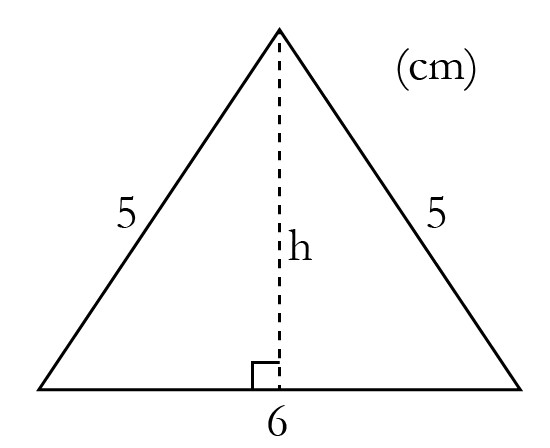
\includegraphics[scale=0.3]{images/34.png} \\
		Satsen om likbent triangel ger att den båda rätvinkliga trianglarna är kongruenta vilket medför att basen för båda är $3cm$.
		Pyth. sats ger att $h=\sqrt{5^2-3^2}=4 \Rightarrow$ arean: $6*4/2=12cm^2$ och omkretsen är $16cm$. \\ \\
		Låt benen vara $y$ och basen $x$ \\ \\
		$h=\sqrt{y^2-(x/2)^2}$ \\
		area: $\dfrac{x*h}{2}=\dfrac{x\sqrt{y^2-(x/2)^2}}{2}=12cm \Leftrightarrow x\sqrt{y^2-(x/2)^2}=24cm$ \\
		omkrets: $2y+x=16cm \Leftrightarrow x=16-2y$
		\begin{align*}
		&(16-2y)\sqrt{y^2-(8-y)^2}=24 \Leftrightarrow
		2(8-y)4\sqrt{y-4}=24 \Leftrightarrow \\
		&(8-y)\sqrt{y-4}=3 \Rightarrow
		(y^2-16y+64)(y-4)=9 \Leftrightarrow \\
		&y^3-4y^2-16y^2+64y+64y-256=9 \Leftrightarrow
		y^3-20y^2+128y-265=0
		\end{align*}
		Ansätter lösning med $x-5$ som faktor från ursprungsfiguren (kan lösas med polynomdivision också): \\
		\[y^3-20y^2+128y-265=(x-5)(x^2+Ax+B)=x^3+(A-5)y^2+(B-5A)y-5B\]
		Identifierar variablerna: \\
		\[\begin{cases}
		A-5=-20 \\
		B-5A=128
		\end{cases}
		\Leftrightarrow
		\begin{cases}
		A=-15 \\
		B=53
		\end{cases}\]
		\[y^3-20y^2+128y-265=(y-5)(y^2-15y+53)\] \\
		$y^2-15y+53=0$ \\
		pq-formeln: \\
		$y=\dfrac{15}{2}\pm\sqrt{\dfrac{15^2-212}{4}}=\dfrac{15\pm\sqrt{13}}{2}$ \\
		$y_1=\dfrac{15+\sqrt{13}}{2} \Rightarrow 
		x=16-15-\sqrt{13} \Rightarrow 
		x < 0 \Rightarrow$ falsk rot \\
		$y_2=\dfrac{15-\sqrt{13}}{2} \Rightarrow x=16-15+\sqrt{13}=1+\sqrt{13}$ \\ \\
		\textbf{Svar:} $x=1+\sqrt{13}$ och $y=\dfrac{15-\sqrt{13}}{2}$
	\end{quotation}
	
	\pagebreak
	\texttt{\tskcol{3.5~~~a) (s.)}}
	\begin{quotation}
		\noindent
		\begin{align*}
		&\dfrac{1}{x-1}+\dfrac{1}{x}+\dfrac{1}{x+1}=0\Leftrightarrow
		\dfrac{x(x+1)+x^2-1+x(x-1)}{x(x^2-1)}=0 \Leftrightarrow \\
		&\dfrac{3x^2-1}{x(x^2-1)}=0\Rightarrow 
		3x^2-1=0 \Leftrightarrow 
		(\sqrt{3}x+1)(\sqrt{3}x-1)=0 \Leftrightarrow
		(x+\frac{1}{\sqrt{3}})(x-\frac{1}{\sqrt{3}})=0
		\end{align*}
		Faktorsatsen ger då: $x_1=-\frac{1}{\sqrt{3}}$ och $x_2=\frac{1}{\sqrt{3}}$
		\\ \\
		\textbf{Svar:} $x_{1,2}=\pm\frac{1}{\sqrt{3}}$
	\end{quotation}
	
	\texttt{\tskcol{~~~~~~b) (s.)}}
	\begin{quotation}
		\noindent
		\begin{align*}
		&\dfrac{1}{x-1}-\dfrac{1}{x-2}=\dfrac{1}{x-3}-\dfrac{1}{x-4}\Leftrightarrow 
		\dfrac{\cancel{x}-2-\cancel{x}+1}{(x-1)(x-2)}=\dfrac{\cancel{x}-4-\cancel{x}+3}{(x-3)(x-4)} \Leftrightarrow \\
		&\dfrac{1}{x^2-3x+2}=\dfrac{1}{x^2-7x+12} \Rightarrow
		\cancel{x^2}-3x+2=\cancel{x^2}-7x+12 \Leftrightarrow \\
		&x=\frac{10}{4}=\frac{5}{2}
		\end{align*}
		\\
		\textbf{Svar:} $x=\frac{5}{2}$
	\end{quotation}
	
	\texttt{\tskcol{~~~~~~c) (s.)}}
	\begin{quotation}
		\noindent
		\begin{align*}
		&\dfrac{1}{x^2-2x}+\dfrac{1}{x^2+3x}=0 \Leftrightarrow 
		\dfrac{\cancel{x}(x+3)+\cancel{x}(x-2)}{x^{\cancel{2}}(x-2)(x+3)}=0 \Rightarrow \\
		&x+3+x-2=0 \Leftrightarrow
		2x+1=0 \Leftrightarrow
		x=-\frac{1}{2}
		\end{align*}
		\\
		\textbf{Svar:} $x=-\frac{1}{2}$
	\end{quotation}
	
	\pagebreak
	\texttt{\tskcol{~~~~~~d) (s.)}}
	\begin{quotation}
		\noindent
		\begin{align*}
		&\dfrac{1}{x+2}-\dfrac{x+2}{x-2}=\dfrac{x^2}{4-x^2}\Leftrightarrow
		\dfrac{x-2-(x+2)^2}{x^2-4}=\dfrac{x^2}{4-x^2} \Rightarrow \\
		&(4-x^2)(-x^2-3x-6)=x^2(x^2-4) \Leftrightarrow \\
		&-\cancel{4x^2}-12x-24+\cancel{x^4}+3x^3+6x^2=\cancel{x^4}-\cancel{4x^2} \Leftrightarrow \\
		&x^3+2x^2-4x-8=0
		\end{align*}
		Gissar en lösning till ekvationen och hittar $x=2$. Ansätter lösning med $x-2$ som faktor (kan lösas med polynomdivision också): 
		\[x^3+2x^2-4x-8=(x-2)(x^2+Ax+B)=x^3+(A-2)x^2+(B-2A)x-2B\]
		Identifierar variabler:
		\[\begin{cases}
		A-2=2 \\
		B-2A=-4
		\end{cases}
		\Leftrightarrow
		\begin{cases}
		A=4 \\
		B=4
		\end{cases}\]
		\[(x-2)(x^2+4x+4)=0\]
		Kvadreringsregeln:
		\[(x-2)(x^2+4x+4)=0\Leftrightarrow 
		(x-2)(x+2)^2=0\]
		Faktorsatsen: $x_1=2$ och $x_{2,3}=-2$.
		Både $2$ och $-2$ är dock falska rötter då de resulterar i nolldivision i ursprungsekvationen.
		\\ \\
		\textbf{Svar:} Ekvationen saknar lösning
	\end{quotation}
	
	\texttt{\tskcol{3.6~~~~~ (s.)}}
	\begin{quotation}
		\noindent
		Formeln för hastighet, sträcka och tid är $s=v*t \Leftrightarrow t=\frac{s}{v}$. Låt $x$ vara båtens hastighet i stillastående vatten. Den totala tiden för resan är tiden dit ($t_1$) plus tiden tillbaka ($t_1$) ($t_1+t_2=t$).
		Hastigheten båten har dit ($v_1$) kan beskrivas som $x-2.4$ och hastigheten hem ($v_2$) som $x+2.4$. $t=2$ och $s=6.4$.
		\[t_1+t_2=t\Leftrightarrow
		\frac{s}{v_1}+\frac{s}{v_2}=t\] \\
		\begin{align*}
		&\frac{6.4}{x-2.4}+\frac{6.4}{x+2.4} = 2 \Leftrightarrow
		\frac{6.4(x+2.4)+6.4(x-2.4)}{(x-2.4)(x+2.4)} = 2 \Leftrightarrow \\
		&6.4(2x+\cancel{2.4-2.4})=2(x^2-2.4^2) \Leftrightarrow
		\cancel{2}*6.4x=\cancel{2}(x^2-2.4^2) \Leftrightarrow \\
		&x^2-6.4x-5.76=0
		\end{align*}
		pq-formeln:
		\[x=3.2\pm\sqrt{10.24+5.76} =3.2\pm\sqrt{16}=3.2\pm 4\]
		$x_1=7.2$ och $x_2=-0.8$. Eftersom hastigheten i uppgiften inte kan vara negativ gäller endast $x_1$
		\\ \\
		\textbf{Svar:} $7.2$ km/h 
	\end{quotation}
	
	\texttt{\tskcol{3.7~~~a) (s.)}}
	\begin{quotation}
		\noindent
		\[\sqrt{x+2}=x \Rightarrow
		x+2=x^2 \Leftrightarrow
		x^2-x-2=0 \]
		pq-formeln: \\
		\[x=\frac{1}{2}\pm\sqrt{\frac{1}{4}+\frac{8}{4}} \Leftrightarrow
		x=\frac{1}{2}\pm\frac{3}{2}\]
		$x_1=2$ \\
		$x_2=-1$ Falsk rot (sätt in i ursprungsekvationen).
		\\ \\
		\textbf{Svar:} $x=2$
	\end{quotation}
	
	\texttt{\tskcol{~~~~~~b) (s.)}}
	\begin{quotation}
		\noindent
		\[\sqrt{x+2}=-x \Rightarrow
		x+2=x^2 \Leftrightarrow
		x^2-x-2=0\]
		pq-formeln: \\
		\[x=\frac{1}{2}\pm\sqrt{\frac{1}{4}+\frac{8}{4}} \Leftrightarrow
		x=\frac{1}{2}\pm\frac{3}{2}\]
		$x_1=2$ Falsk rot (sätt in i ursprungsekvationen). \\
		$x_2=-1$
		\\ \\
		\textbf{Svar:} $x=-1$
	\end{quotation}
	
	\texttt{\tskcol{~~~~~~c) (s.)}}
	\begin{quotation}
		\noindent
		\begin{align*}
		&x-\sqrt{x-2}=4 \Leftrightarrow
		\sqrt{x-2}=x-4 \Rightarrow
		x-2=(x-4)^2 \Leftrightarrow \\
		&x-2=x^2-8x+16 \Leftrightarrow
		x^2-9x+18=0
		\end{align*}
		pq-formeln: \\
		\[x=\frac{9}{2}\pm\sqrt{\frac{81}{4}-\frac{72}{4}} \Leftrightarrow
		x=\frac{9}{2}\pm\frac{3}{2}\]
		$x_1=6$ \\
		$x_2=3$ Falsk rot (sätt in i ursprungsekvationen).
		\\ \\
		\textbf{Svar:} $x=6$
	\end{quotation}
	
	\texttt{\tskcol{3.8~~~a) (s.)}}
	\begin{quotation}
		\noindent
		\[\sqrt{x+2}=\sqrt{2x+1} \Rightarrow
		x+2=2x+1 \Leftrightarrow
		x=1\]
		\\
		\textbf{Svar:} $x=1$
	\end{quotation}
	
	\pagebreak
	\texttt{\tskcol{~~~~~~b) (s.)}}
	\begin{quotation}
		\noindent
		\[\sqrt{3x+2}=\sqrt{2x+1} \Rightarrow
		3x+2=2x+1 \Leftrightarrow
		x=-1 \text{~~~Falsk rot.}\]
		\\
		\textbf{Svar:} Ekvationen saknar lösning
	\end{quotation}
	
	\texttt{\tskcol{~~~~~~c) (s.)}}
	\begin{quotation}
		\noindent
		\[\sqrt{x+2}=\sqrt{x} \Rightarrow
		x+2=x \Leftrightarrow
		2=0 \text{~~~Ej ekvivalent.}\]
		\\
		\textbf{Svar:} Ekvationen saknar lösning
	\end{quotation}
		
	\texttt{\tskcol{~~~~~~d) (s.)}}
	\begin{quotation}
		\noindent
		\[\sqrt{x-2}\sqrt{x+3}=x \Rightarrow
		(x-2)(x+3)=x^2 \Leftrightarrow
		\cancel{x^2}+x-6=\cancel{x^2} \Leftrightarrow
		x=6\]
		\\
		\textbf{Svar:} $x=6$
	\end{quotation}
	
	\texttt{\tskcol{~~~~~~e) (s.)}}
	\begin{quotation}
		\noindent
		\begin{align*}
		&(3-\sqrt{x})(3+\sqrt{x})=8\sqrt{x} \Leftrightarrow
		9-x=8\sqrt{x} \Rightarrow \\
		&x^2-18x+81=64x \Leftrightarrow
		x^2-82x+81=0
		\end{align*}
		pq-formeln: \\
		\[x=41\pm\sqrt{41^2-81}=41\pm40\]
		$x_1=81$ falsk rot. \\
		$x_2=1$
		\\ \\
		\textbf{Svar:} $x=1$
	\end{quotation}
		
	\texttt{\tskcol{~~~~~~f) (s.)}}
	\begin{quotation}
		\noindent
		\begin{align*}
		&\sqrt{x}=\dfrac{3}{\sqrt{x}}+\sqrt{3+x} \Leftrightarrow
		x=3+\sqrt{x(3+x)} \Leftrightarrow
		x-3=\sqrt{3x+x^2} \Rightarrow \\
		&\cancel{x^2}-6x+9=3x+\cancel{x^2} \Leftrightarrow
		9x=9 \Leftrightarrow
		x=1 \text{~~~Falsk rot.}
		\end{align*}
		\\
		\textbf{Svar:} Lösning saknas
	\end{quotation}
	
	\subsection*{Ekvationer}
	
	\texttt{\tskcol{3.9~~~~~ (s.)}}
	\begin{quotation}
		\noindent
		$2<3 \Leftarrow$ är ''2 \textbf{mindre} än 3''? Ja \\
		$2 \le 3 \Leftarrow$ är ''2 \textbf{mindre} eller lika med 3''? Ja \\
		$2 \le 2 \Leftarrow$ är ''2 mindre eller \textbf{lika med} 2''? Ja 
		\\ \\
		\textbf{Svar:} Alla tre
	\end{quotation}
	
	\texttt{\tskcol{3.10~~~~ (s.)}}
	\begin{quotation}
		\noindent
		Nedan visar jag min tankeprocess för att lösa uppgiften.
		\[\frac{2}{0.02}=
		\frac{2}{2}*\frac{1}{10^{-2}}=
		1*10^2=
		100\]
		\[\frac{31}{0.2}=
		\frac{31}{2}*\frac{1}{10^{-1}}=
		15.5*10=
		155\]
		\[\frac{0.00009}{0.000006}=
		\frac{9}{6}*\frac{10^{-5}}{10^{-6}}=
		1.5*10=
		15\]
		\\ \\
		\textbf{Svar:} $\dfrac{0.00009}{0.000006}<\dfrac{2}{0.02}<\dfrac{31}{0.2}$
	\end{quotation}
	
	\texttt{\tskcol{3.11~~a) (s.)}}
	\begin{quotation}
		\noindent
		$3x+1<2 \Leftrightarrow
		3x<1 \Leftrightarrow
		x<\frac{1}{3}$
		\\ \\
		\textbf{Svar:} $x<\frac{1}{3}$
	\end{quotation}
	
	\texttt{\tskcol{~~~~~~b) (s.)}}
	\begin{quotation}
		\noindent
		$-3x+2\le1 \Leftrightarrow
		-3x\le-1 \Leftrightarrow
		x\ge\frac{1}{3}$
		\\ \\
		\textbf{Svar:} $x\ge\frac{1}{3}$
	\end{quotation}
	
	\texttt{\tskcol{~~~~~~c) (s.)}}
	\begin{quotation}
		\noindent
		$3x+1>4x+5 \Leftrightarrow
		x<-4$
		\\ \\
		\textbf{Svar:} $x<-4$
	\end{quotation}
	
	\texttt{\tskcol{~~~~~~d) (s.)}}
	\begin{quotation}
		\noindent
		$(x-3)(x+3)\le x^2 \Leftrightarrow
		\cancel{x^2}-9 \le \cancel{x^2} \Leftrightarrow
		-9 \le 0 \Rightarrow x\in\mathbb{R}$
		\\ \\
		\textbf{Svar:} $x\in\mathbb{R}$
	\end{quotation}
	
	\pagebreak
	\texttt{\tskcol{3.12~~a) (s.)}}
	\begin{quotation}
		\noindent
		Använd en teckentabell och hitta intervallet/n som ger positiva värden.
		
		 \[\dfrac{x+4}{x-1}>0\] \\
		\begin{tabular}{c|c|c|c|c|c}
			$x$ & & $-4$ & & $1$ & \\ \hline
			$x+4$              & $-$ & $0$ & $+$ & $+$ & $+$ \\
			$x-1$              & $-$ & $-$ & $-$ & $0$ & $+$ \\ \hline
			$\dfrac{x+4}{x-1}$ & $+$ & $0$ & $-$ &$\wr$& $+$ 
		\end{tabular} \\ \\
		\textbf{Svar:} $x>1$ eller $x<-4$
	\end{quotation}
	
	\texttt{\tskcol{~~~~~~b) (s.)}}
	\begin{quotation}
		\noindent
		Utnyttja teckentabellen i förra uppgiften men ta intervallet som ger negativa värden.
		
		\[\dfrac{x+4}{x-1}<0\]
		\\
		\textbf{Svar:} teckenschemat i \texttt{\tskcol{a)}} ger: $-4<x<1$
	\end{quotation}
	
	\texttt{\tskcol{~~~~~~c) (s.)}}
	\begin{quotation}
		\noindent
		Använd en teckentabell och hitta intervallet/n som ger negativa värden.
		\[\dfrac{x+1}{x(x-1)}<0\] \\
		\begin{tabular}{c|c|c|c|c|c|c|c}
			$x$ & & $-1$ & & $0$ & & $1$ & \\ \hline
			$x+1$                  & $-$ & $0$ & $+$ & $+$ & $+$ & $+$ & $+$ \\
			$x$                    & $-$ & $-$ & $-$ & $0$ & $+$ & $+$ & $+$ \\
			$x-1$                  & $-$ & $-$ & $-$ & $-$ & $-$ & $0$ & $+$ \\ \hline
			$\dfrac{x+1}{x(x-1)}$  & $-$ & $0$ & $+$ &$\wr$& $-$ &$\wr$& $+$ \\
		\end{tabular}
		\\ \\
		\textbf{Svar:} $x<-1$ eller $0<x<1$
	\end{quotation}
	
	\texttt{\tskcol{~~~~~~d) (s.)}}
	\begin{quotation}
		\noindent
		Använd en teckentabell och hitta intervallet/n som ger positiva värden.
		\[(x+2)(2x-1) > 0\] \\
		\begin{tabular}{c|c|c|c|c|c}
			$x$ & & $-2$ & & $1/2$ & \\ \hline
			$x+2$         & $-$ & $0$ & $+$ & $+$ & $+$ \\
			$2x-1$        & $-$ & $-$ & $-$ & $0$ & $+$ \\ \hline
			$(x+2)(2x-1)$ & $+$ & $0$ & $-$ &$\wr$& $+$ 
		\end{tabular}
		\\ \\
		\textbf{Svar:} $x<-2$ eller $x>1/2$
	\end{quotation}
	
	\pagebreak
	\texttt{\tskcol{3.13~~~~ (s.)}}
	\begin{quotation}
		\noindent
		Skriv om skillnaden så att högerledet blir noll och allt i vänsterledet hamnar på samma bråkstreck. Använd sedan en teckentabell och hitta intervallet/n som ger negativa värden.
		
		\[\dfrac{3x+1}{x+2}<2 \Leftrightarrow
		\dfrac{3x+1-2(x+2)}{x+2}<0 \Leftrightarrow
		\dfrac{x-3}{x+2}<0\] \\
		\begin{tabular}{c|c|c|c|c|c}
			$x$ & & $-2$ & & $3$ & \\ \hline
			$x-3$              & $-$ & $-$ & $-$ & $0$ & $+$ \\
			$x+2$              & $-$ & $0$ & $+$ & $+$ & $+$ \\ \hline
			$\dfrac{x-3}{x+2}$ & $+$ &$\wr$& $-$ & $0$ & $+$ 
		\end{tabular}
		\\ \\
		\textbf{Svar:} $-2<x<3$
	\end{quotation}
	
	\texttt{\tskcol{3.14~~a) (s. 44-45)}}
	\begin{quotation}
		\noindent
		Se sidorna 44-45 i läroboken för förklaring till varför det funkar såhär.
		\[\dfrac{x^2+1}{x}<x\]
		\begin{align*}
		&\text{om } x>0\text{:} &\dfrac{x^2+1}{x}<x &\Leftrightarrow &\cancel{x^2}+1<\cancel{x^2} &\Leftrightarrow &1<0 \\
		&\text{om } x<0\text{:} &\dfrac{x^2+1}{x}<x &\Leftrightarrow &\cancel{x^2}+1>\cancel{x^2} &\Leftrightarrow &1>0
		\end{align*}
		$1<0$ är alltid sant vilket innebär att skillnaden gäller för alla $x$ mindre än noll.
		\\ \\
		\textbf{Svar:} $x<0$ 
	\end{quotation}
	
	\texttt{\tskcol{~~~~~~b) (s.)}}
	\begin{quotation}
		\noindent
		\\ \\
		\textbf{Svar:} 
	\end{quotation}
	
	\texttt{\tskcol{~~~~~~c) (s.)}}
	\begin{quotation}
		\noindent
		\\ \\
		\textbf{Svar:} 
	\end{quotation}
	
	\texttt{\tskcol{3.15~~a) (s.)}}
	\begin{quotation}
		\noindent
		\\ \\
		\textbf{Svar:} 
	\end{quotation}
	
	\texttt{\tskcol{~~~~~~b) (s.)}}
	\begin{quotation}
		\noindent
		\\ \\
		\textbf{Svar:} 
	\end{quotation}
	
	\texttt{\tskcol{~~~~~~c) (s.)}}
	\begin{quotation}
		\noindent
		\\ \\
		\textbf{Svar:} 
	\end{quotation}
	
	\texttt{\tskcol{3.16~~~~ (s.)}}
	\begin{quotation}
		\noindent
		\\ \\
		\textbf{Svar:} 
	\end{quotation}
	
	\texttt{\tskcol{3.17~~a) (s.)}}
	\begin{quotation}
		\noindent
		\\ \\
		\textbf{Svar:} 
	\end{quotation}
	
	\texttt{\tskcol{~~~~~~b) (s.)}}
	\begin{quotation}
		\noindent
		\\ \\
		\textbf{Svar:} 
	\end{quotation}
	
\end{document}